\chapter{Detalhes da Implementação}

\section{Introdução}

Este capítulo irá descrever detalhes da implementação do sistema de treinamento e inserção automática desenvolvida. Para atender as especificações necessárias, uma aplicação foi desenvolvida para facilitar facilitar o treinamento, assim como para automatizar a geração de modelos tridimensionais de fotos inseridas para treinamento.

\section{Sistema de Inserção}
\label{sec:sistema-imersao}

Inserir informações da aplicação
%The web server application\footnote{https://www.swheelchairth.com.br:8443/servletserver/} is running over Apache-Tomcat-7.0.78 with MySQL Database$^{\textregistered}$ using Java$\texttrademark$ language. This system platform is based in the MVC architecture and each component was describe in Figure \ref{fig:mvc-layersArch}, in Section \ref{sec:webserverApp}. It makes easy to incorporate different libraries and frameworks (Multi-WebRTC, JSArtoolkit, Boostrap, Web Graphics Library (WebGL) and GL Transmission Format (GLTF) models) to build a reliable web application. Servlets are used in MVC model to control events that come from JSP pages, through POST, GET requests and also external data coming from sockets. In this system, there are two basic actors' roles: therapist and patient. Before initiating all explanations about the implementation details between the front-end and backend, the existent folders (Figures \ref{fig:folders01} and \ref{fig:folders02}), servlets (Figure \ref{fig:servlets01}), files (Figures \ref{fig:files01}, \ref{fig:files02}, \ref{fig:files03} and \ref{fig:files04}) and tables (Figure \ref{fig:tablesDiagram}) are listed.  

%\begin{figure}[!htbp]
%\center
%\begin{minipage}{0.495\linewidth}
%\center
%\captionsetup{justification=centering,margin=0cm,font=small}
%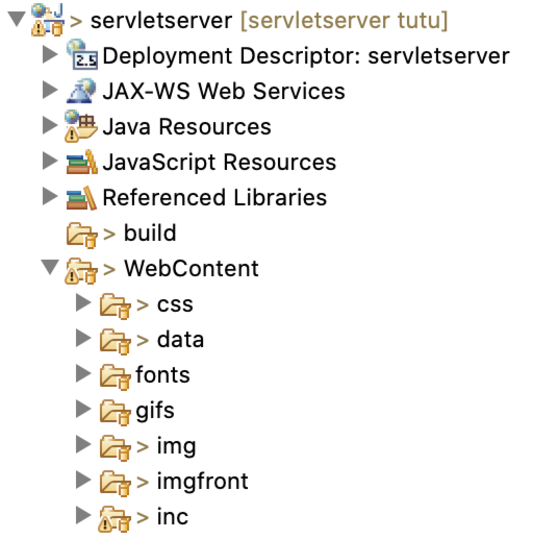
\includegraphics[width=0.8\linewidth]{img/cap5/folders01}
%\caption{Project folders part-one} \label{fig:folders01}
%\end{minipage}
%\begin{minipage}{0.495\linewidth}
%\center
%\captionsetup{justification=centering,margin=0cm,font=small}
%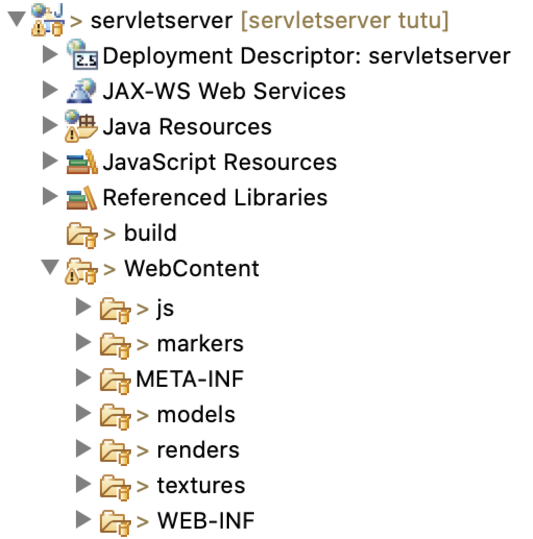
\includegraphics[width=0.8\linewidth]{img/cap5/folders02}
%\caption{Project folders part-two} \label{fig:folders02}
%\end{minipage}
%\end{figure}
%
%\begin{figure}[!hbt]
%\begin{center}
%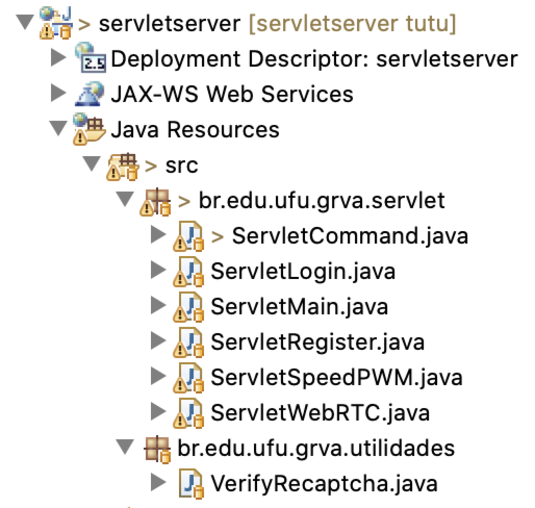
\includegraphics[width=0.4\linewidth]{img/cap5/servlets01}
%\caption{Java Servlets} \label{fig:servlets01}
%\end{center}
%\end{figure}
%
%\begin{figure}[!htbp]
%\center
%\begin{minipage}{0.495\linewidth}
%\center
%\captionsetup{justification=centering,margin=0cm,font=small}
%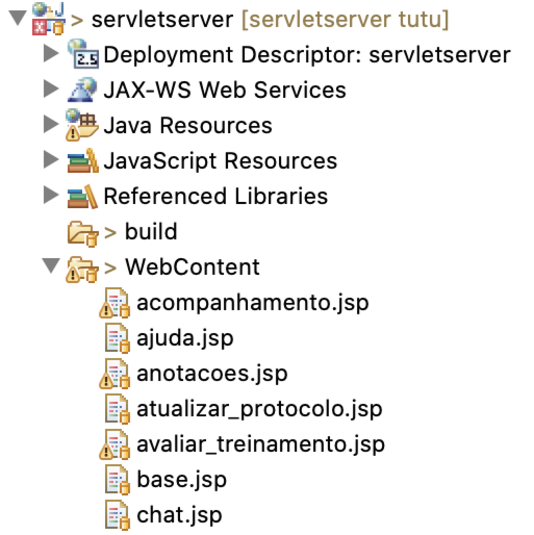
\includegraphics[width=0.8\linewidth]{img/cap5/files01}
%\caption{Files part-one} \label{fig:files01}
%\end{minipage}
%\begin{minipage}{0.495\linewidth}
%\center
%\captionsetup{justification=centering,margin=0cm,font=small}
%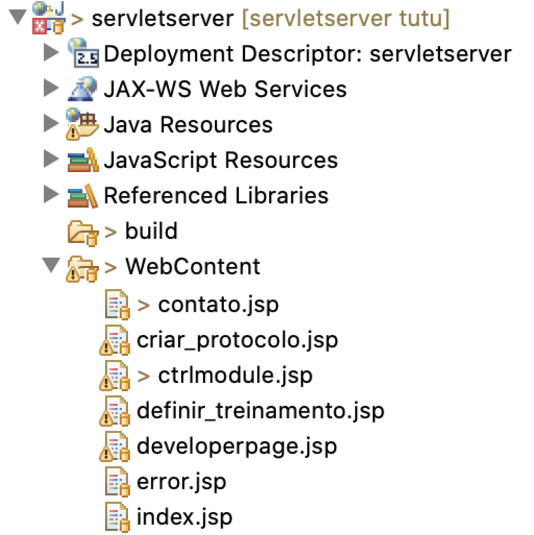
\includegraphics[width=0.8\linewidth]{img/cap5/files02}
%\caption{Files part-two} \label{fig:files02}
%\end{minipage}
%\center
%\begin{minipage}{0.495\linewidth}
%\center
%\captionsetup{justification=centering,margin=0cm,font=small}
%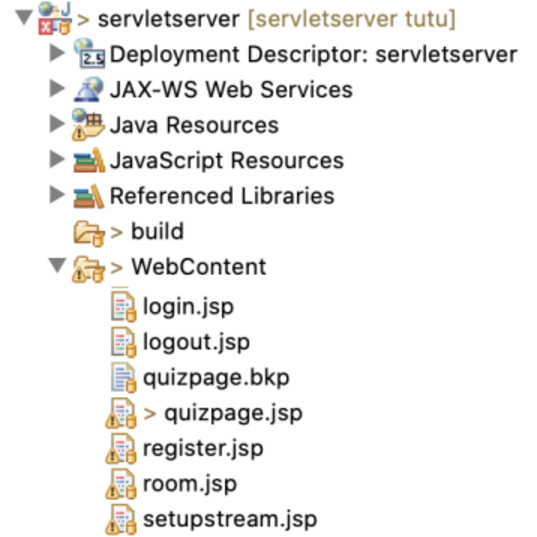
\includegraphics[width=0.8\linewidth]{img/cap5/files03}
%\caption{Files part-three} \label{fig:files03}
%\end{minipage}
%\begin{minipage}{0.495\linewidth}
%\center
%\captionsetup{justification=centering,margin=0cm,font=small}
%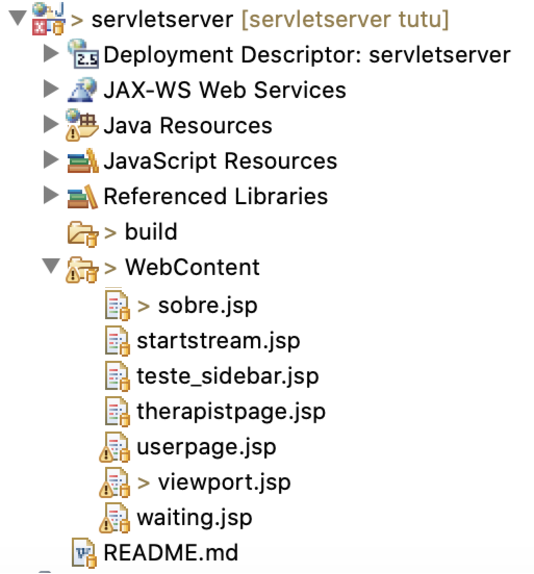
\includegraphics[width=0.8\linewidth]{img/cap5/files04}
%\caption{Files part-four} \label{fig:files04}
%\end{minipage}
%\end{figure}
%
%
%In the next sections, the explanations containing the implementation details, will follow a flow that starts from each view page, connected with sequence action diagram, the related files (scripts, models, animations), as well as, each controller (Servlet) handler. Providing tips on how to reproduce the test environment, which will be freely shared with the community under the restrictions of the GNU General Public License (GPL).
%
%\begin{figure}[!hbt]
%\begin{center}
%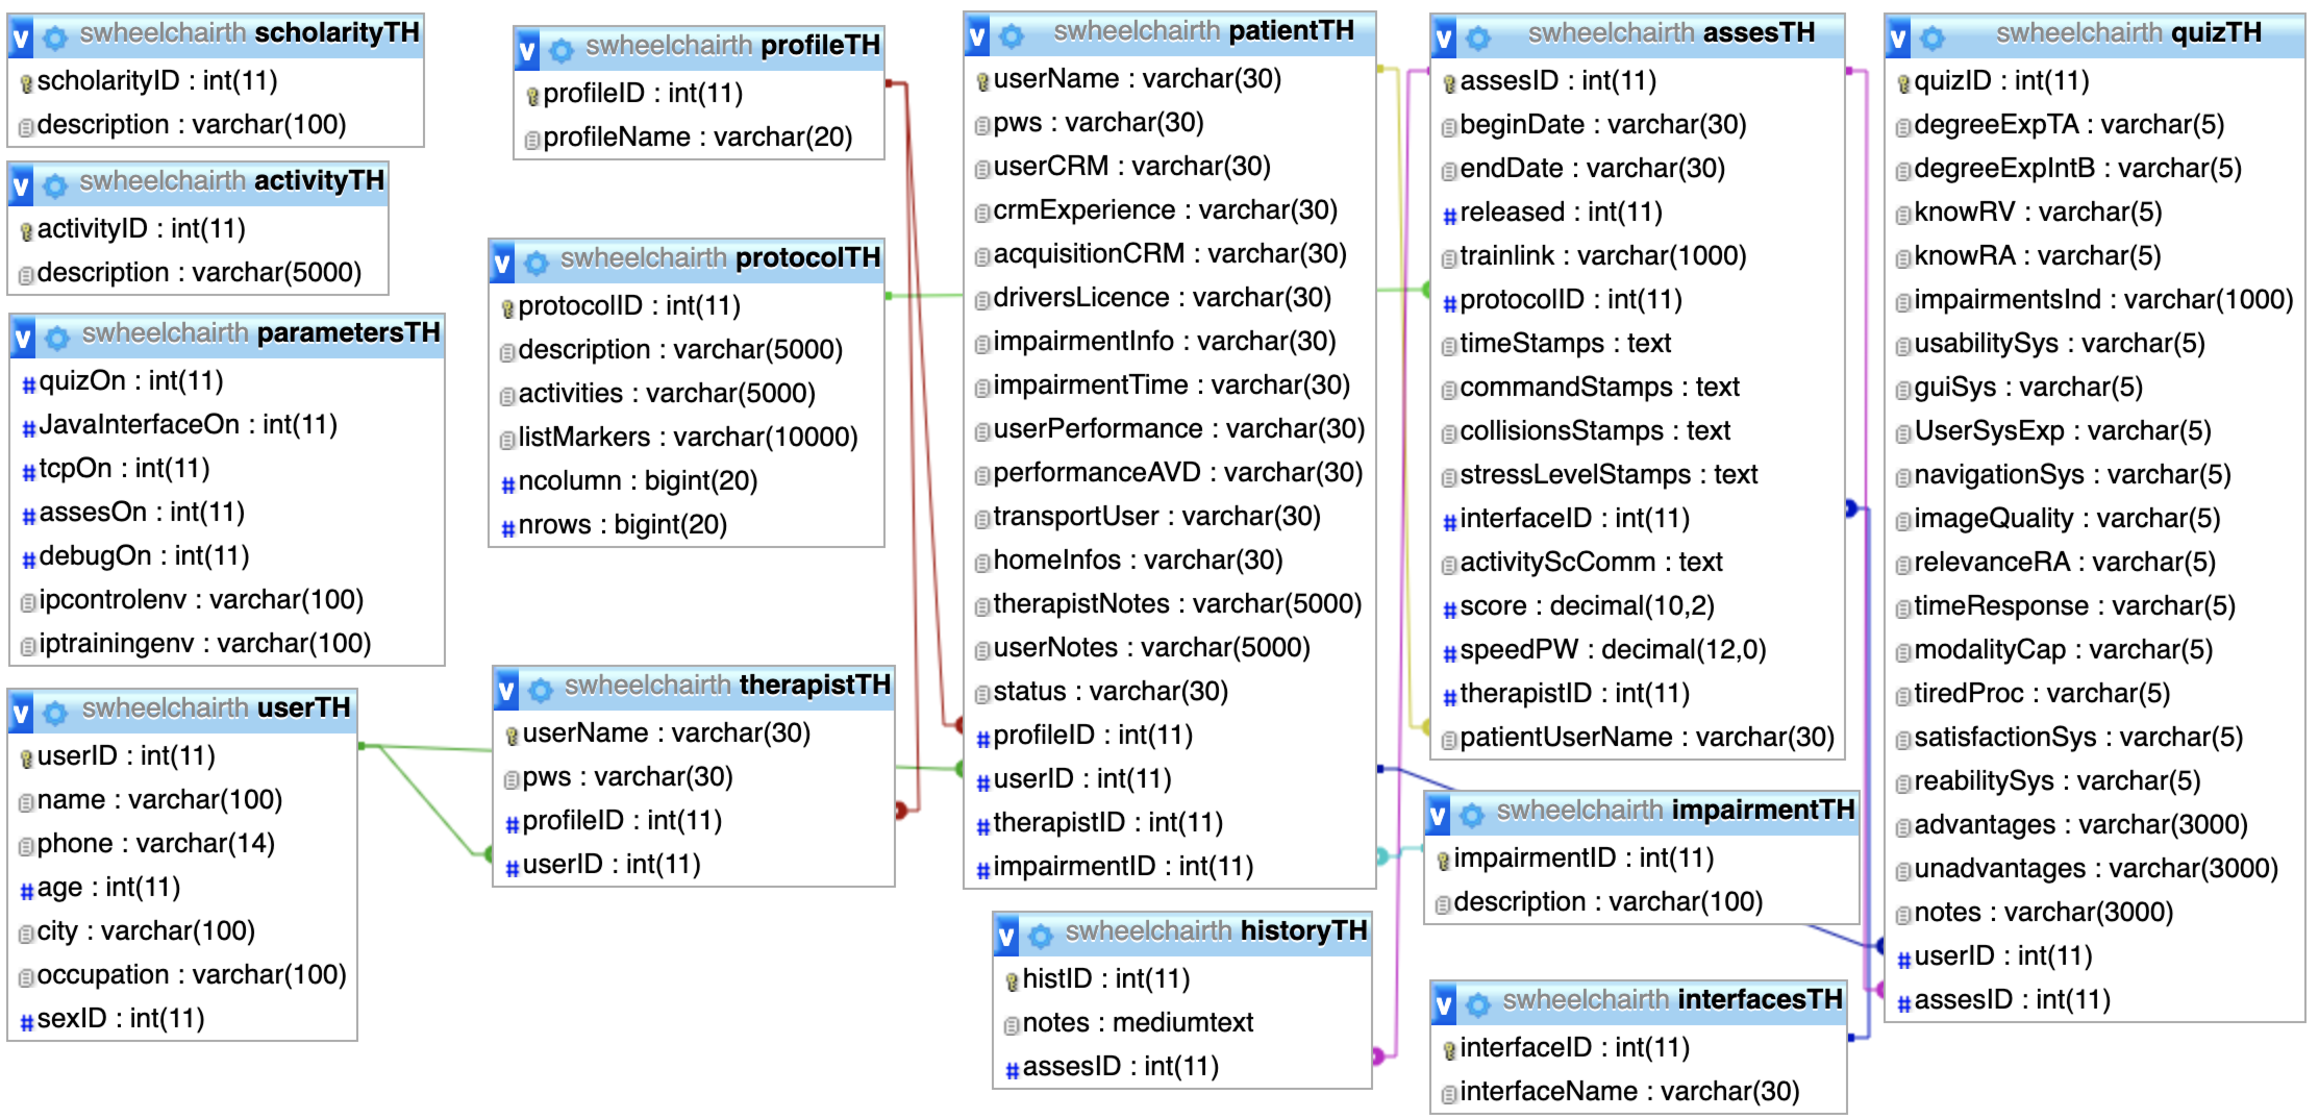
\includegraphics[width=1\linewidth]{img/cap5/tablesDiagram}
%\caption{Tables diagram} \label{fig:tablesDiagram}
%\end{center}
%\end{figure}
%
%\subsection{Home page}
%\label{sec:homepage}
%
%Figure \ref{fig:mainFrontSite} shown the system home page, stored on index.jsp file. 
%
%\begin{figure}[!hbt]
%\begin{center}
%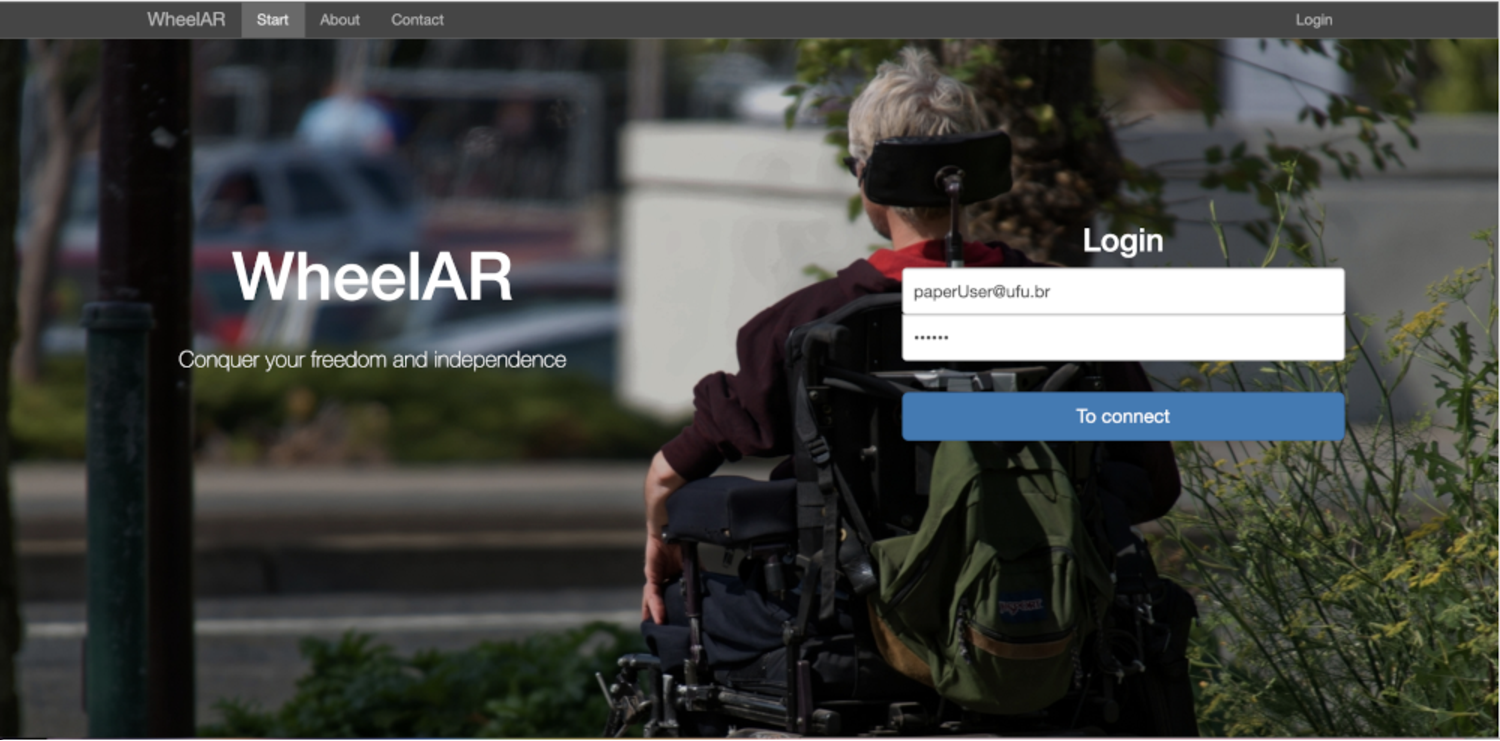
\includegraphics[width=1\linewidth]{img/cap5/mainFrontSite}
%\caption{AR Wheel home page} \label{fig:mainFrontSite}
%\end{center}
%\end{figure}
%
%The navigation bar on top is included on file by the special Java tag below. It is responsible for updating respective headers and footers on view pages, with different contents like navigation menu bar. It has two kinds of files that can be used distinctly: one when the user is not logged into the system and the other one when he/she is logged. \newline
%
%\begin{lstlisting}[frame=single,language=Java]  % Start your code-block
%include file="inc/header.jsp"
%<%@ include file="inc/header.jsp" %>
%\end{lstlisting}
%
%In this home page, the users does not need to be logged into the system to access the actions on top. Otherwise, if the user profile is ``therapist'' the headerLogged.jsp file, stored in ``inc'' folder is charged, or, if the user profile is ``patient'' the header\_logged\_user.jsp, is charged with specific menu bar actions.
%
%From this view page, the  user still can access other static contents from the  ``About'' and ``Contact'' link, on top, stored in files  (contato and sobre).jsp. A 360$^{\circ}$ image preview (Figure \ref{fig:roomView}) from the remote training site was built, using the ``A-Frame''\footnote{https://aframe.io/} framework for building VR experience. For creating this effect, the following embedded body HTML tag is presented. This view page is stored in room.jsp file and can be accessed from the ``Contact'' link.
%\newline
%
%\begin{lstlisting}[frame=single,language=HTML]  % Start your code-block
%<script src="https://aframe.io/releases/0.8.2/aframe.min.js"></script>
%</head>
%<body>
%  <a-scene> 
%    <a-sky src="imgfront/sala_fisica/IMG_20190114_135100.JPG" 
%   rotation=0 -130 0>
%    </a-sky>
%  </a-scene>
%</body>
%\end{lstlisting}
%
%
%\subsubsection{Logging in UC action}
%\label{sec:logginSystem}
%
%These last pages do not interact with the backend. However, there is still the action of logging in to the system (stored in file login.jsp), which is extremely important, as it ensures that each UC is implemented and executed correctly in the future.
%
%Based on the SD actions in Figures \ref{fig:UMLSD-UserWebCase01} and \ref{fig:UMLSD-TherapistWebCase01}, the ``loginButton'' action is sent to the ``ServletLogin'', which checks whether the existing credentials are valid. Whether the credentials are valid, the sessions variables (user name and profile) and databases (user status: online) values, are updated and then, the users are redirected to their respective viewing pages, with the appropriate headers and navigation bar, in agreement with the UC in Figures \ref{subfig:userCaseWeb} and \ref{fig:therapistCases}. Otherwise, it updates user status: offline (table patientTH) and redirects the user back to the login view page (stored as login.jsp file). 
%
%\subsection{User session}
%
%Once the user has logged into the system, the user view page (stored as userpage.jsp) that is implements the user web UC actions (Figure \ref{subfig:userCaseWeb}) is shown in Figure \ref{fig:tUserSession}.
%
%\begin{figure}[!hbt]
%\begin{center}
%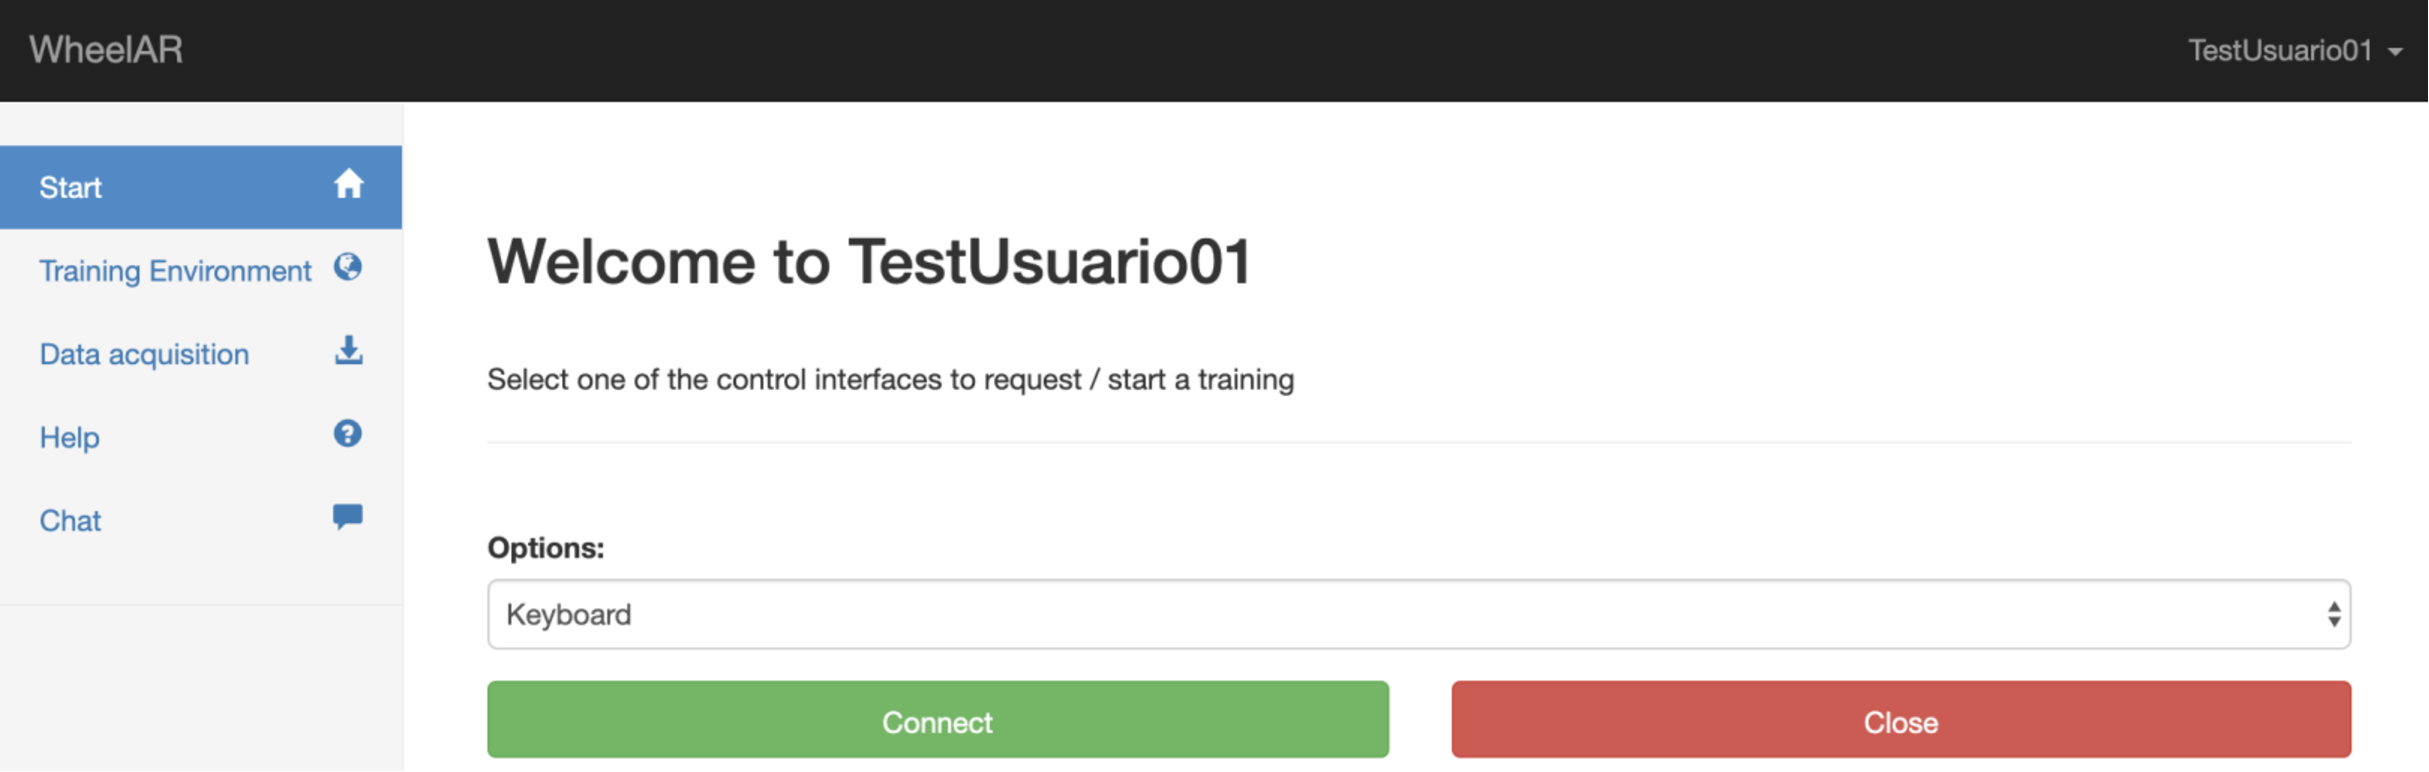
\includegraphics[width=0.95\linewidth]{img/cap5/tUserSession}
%\caption{Main user page interaction} \label{fig:tUserSession}
%\end{center}
%\vspace{-15pt}
%\end{figure}
%
%As mentioned before, specific headers are loaded to allow the preview of the navigation menu bar. From the ``Connect'' button, a new training request is performed and forward to ``ServletCommand''. The Java Servlets implemented are prepared to recognize each button action and proceed with each SD (Figure \ref{fig:UMLSD-UserWebCase01}) action. Then,  if it has no remaining training to be accomplished, a new one is registered (assessTH table). Some credentials are updated (user status: waiting and training ID) into the session and the user is redirected to ``Waiting.jsp'' view page. 
%
%\subsubsection{Waiting view page}
%\label{sec:waitingVP}
%
%This view page (Figure \ref{fig:tWaitingSession} and stored as waiting.jsp) is as system action used to instruct the users of the virtual objects and also checks when a training session is ready. 
%
%\begin{figure}[!hbt]
%\begin{center}
%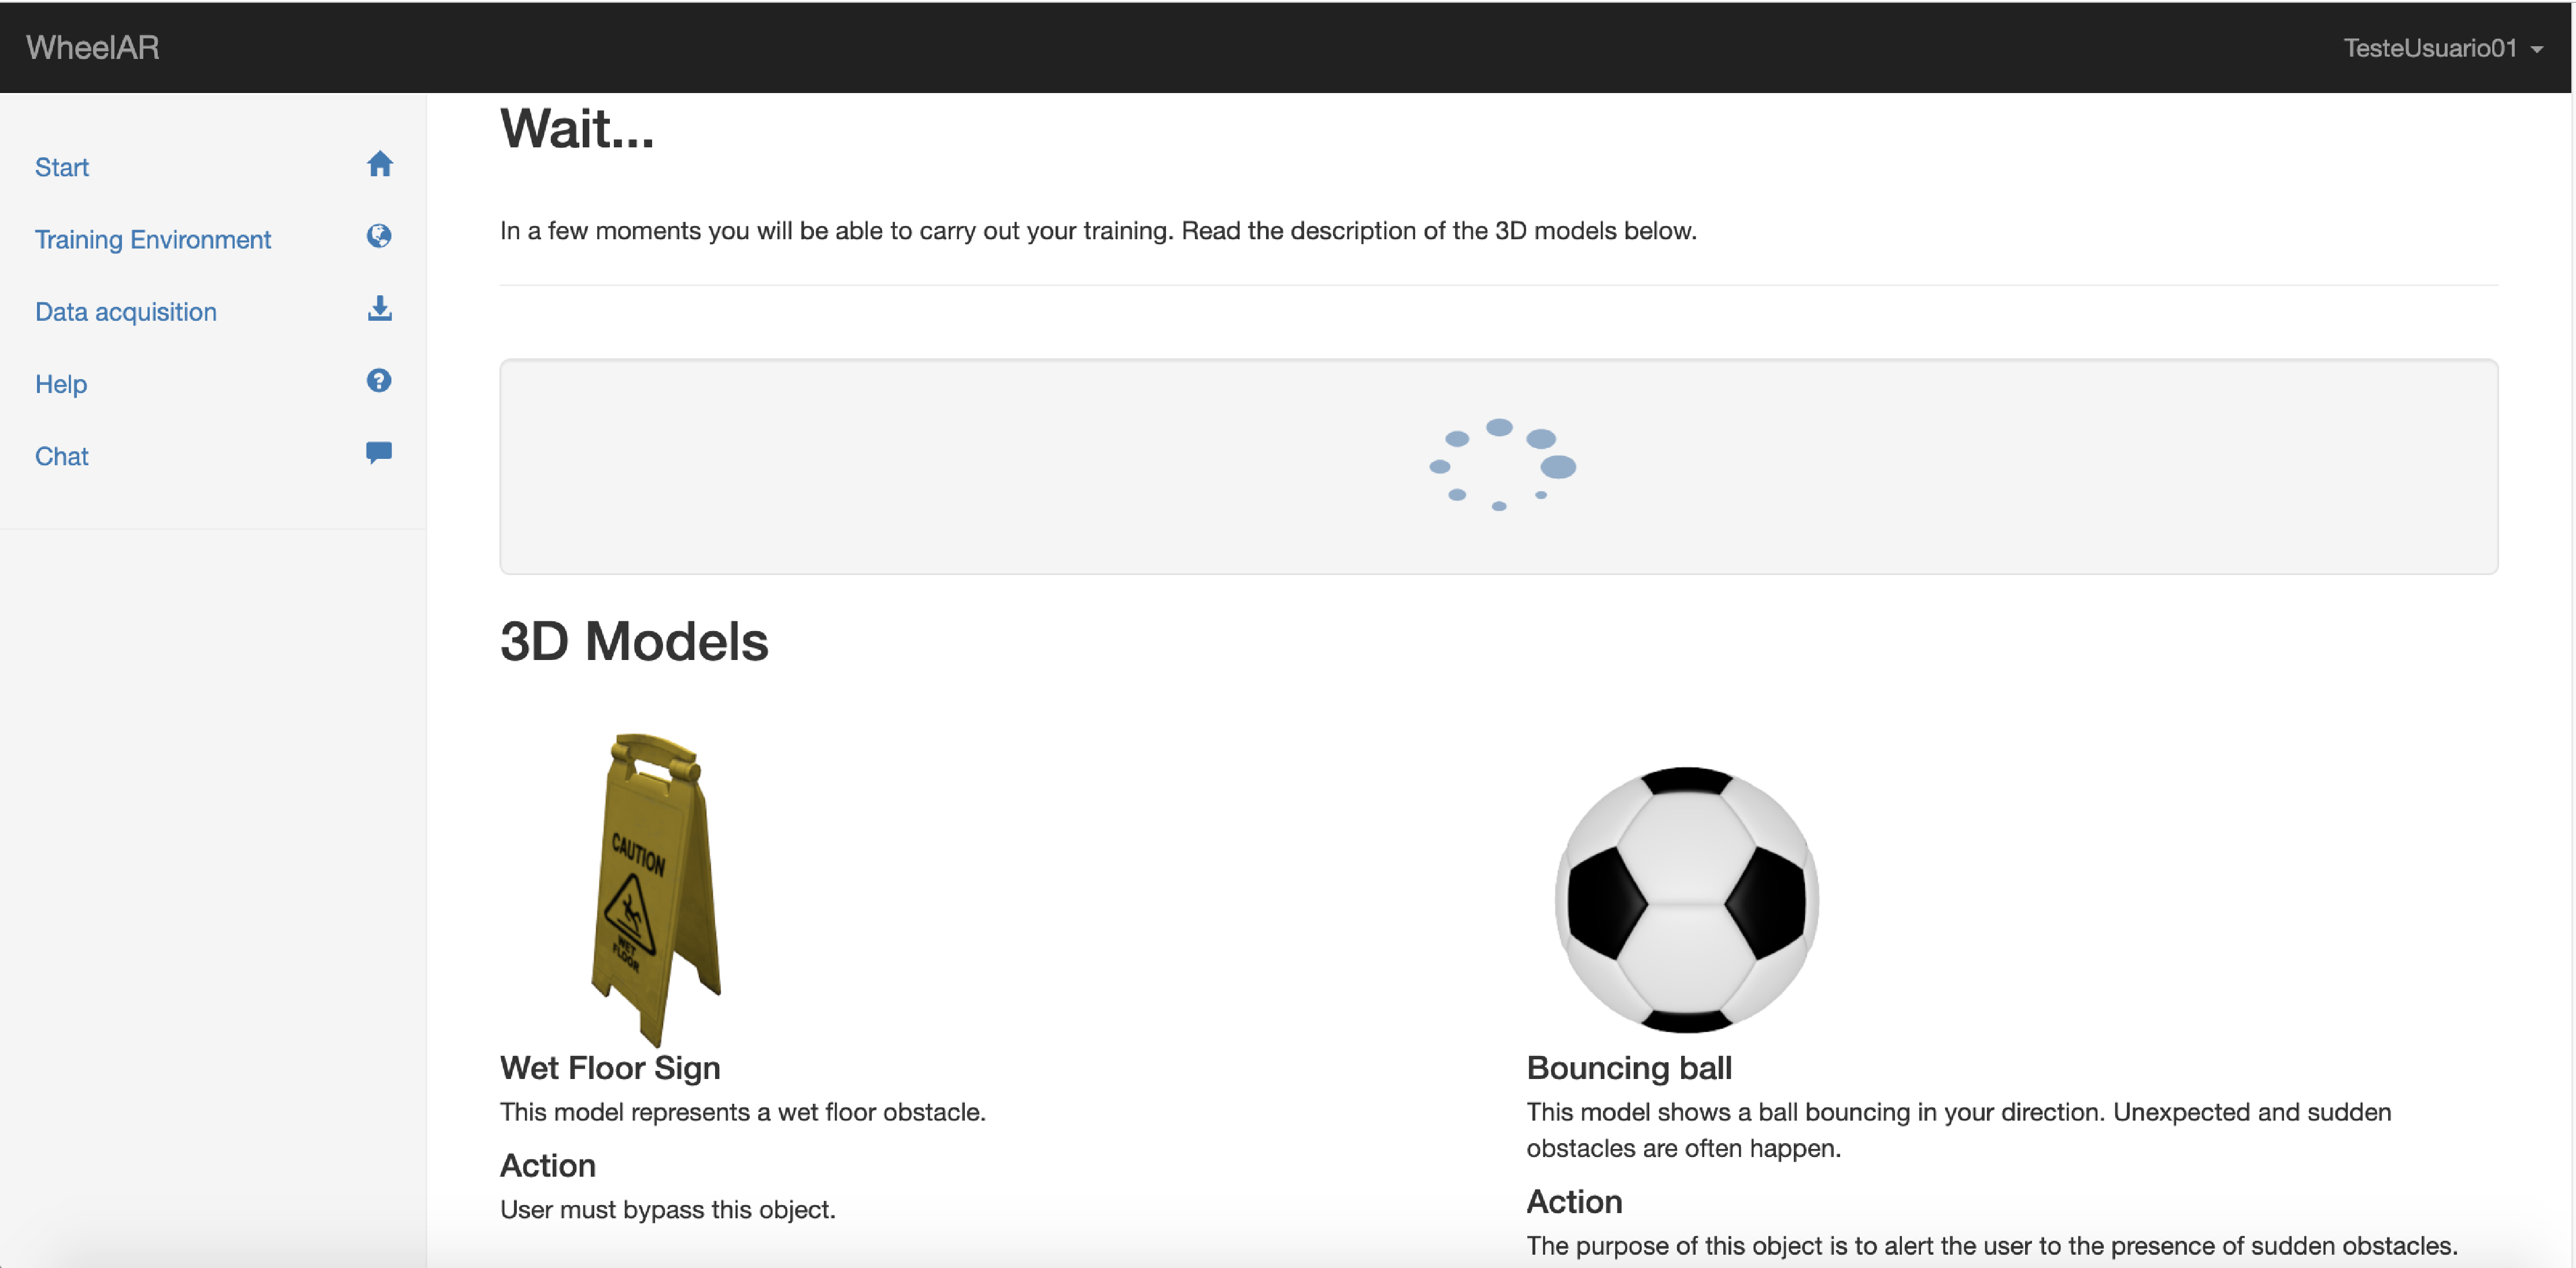
\includegraphics[width=0.95\linewidth]{img/cap5/tWaitingSession}
%\caption{Waiting release training page} \label{fig:tWaitingSession}
%\end{center}
%\vspace{-15pt}
%\end{figure}
%
%An embedded Java code block is executed periodically to check if a training URL was already defined. After, if a new training protocol were requested, all training protocol data from table protocolTH (protocolID, description, activities, listMarkers and (column and rows) number) is updated into the session. As soon as the therapist initiated the remote video stream, this means that both user and therapist are ready to interact with the training site. From this moment, all command information received and its timestamp are recorded in the ``timeStamps'' and ``commandStamps'' columns of the assessTH table. These information are separated by ``;'' and ``,'' as shown by Figure \ref{fig:cmdAndTime-Stamps}.
%
%Then, the users are redirected to another view page ``ViewPort'' (stored as viewport.jsp) that allows the users and therapist to perform their actions and also to have an augmented feedback from the training site.
%
%\begin{figure}[!hbt]
%\begin{center}
%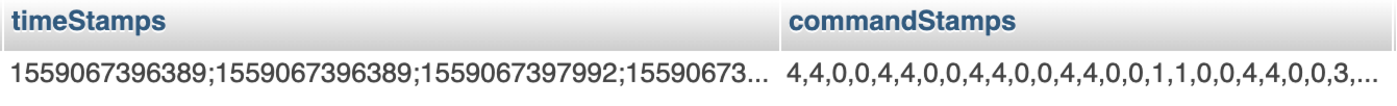
\includegraphics[width=1\linewidth]{img/cap5/cmdAndTime-Stamps}
%\caption{Data information collecting} \label{fig:cmdAndTime-Stamps}
%\end{center}
%\vspace{-15pt}
%\end{figure}
%
%\subsubsection{ViewPort}
%\label{sec:viewPortUser} 
%
%Figure \ref{fig:tViewPortUser} illustrate the ``Viewport'' view page, to a patient profile. 
%
%\begin{figure}[!hbt]
%\begin{center}
%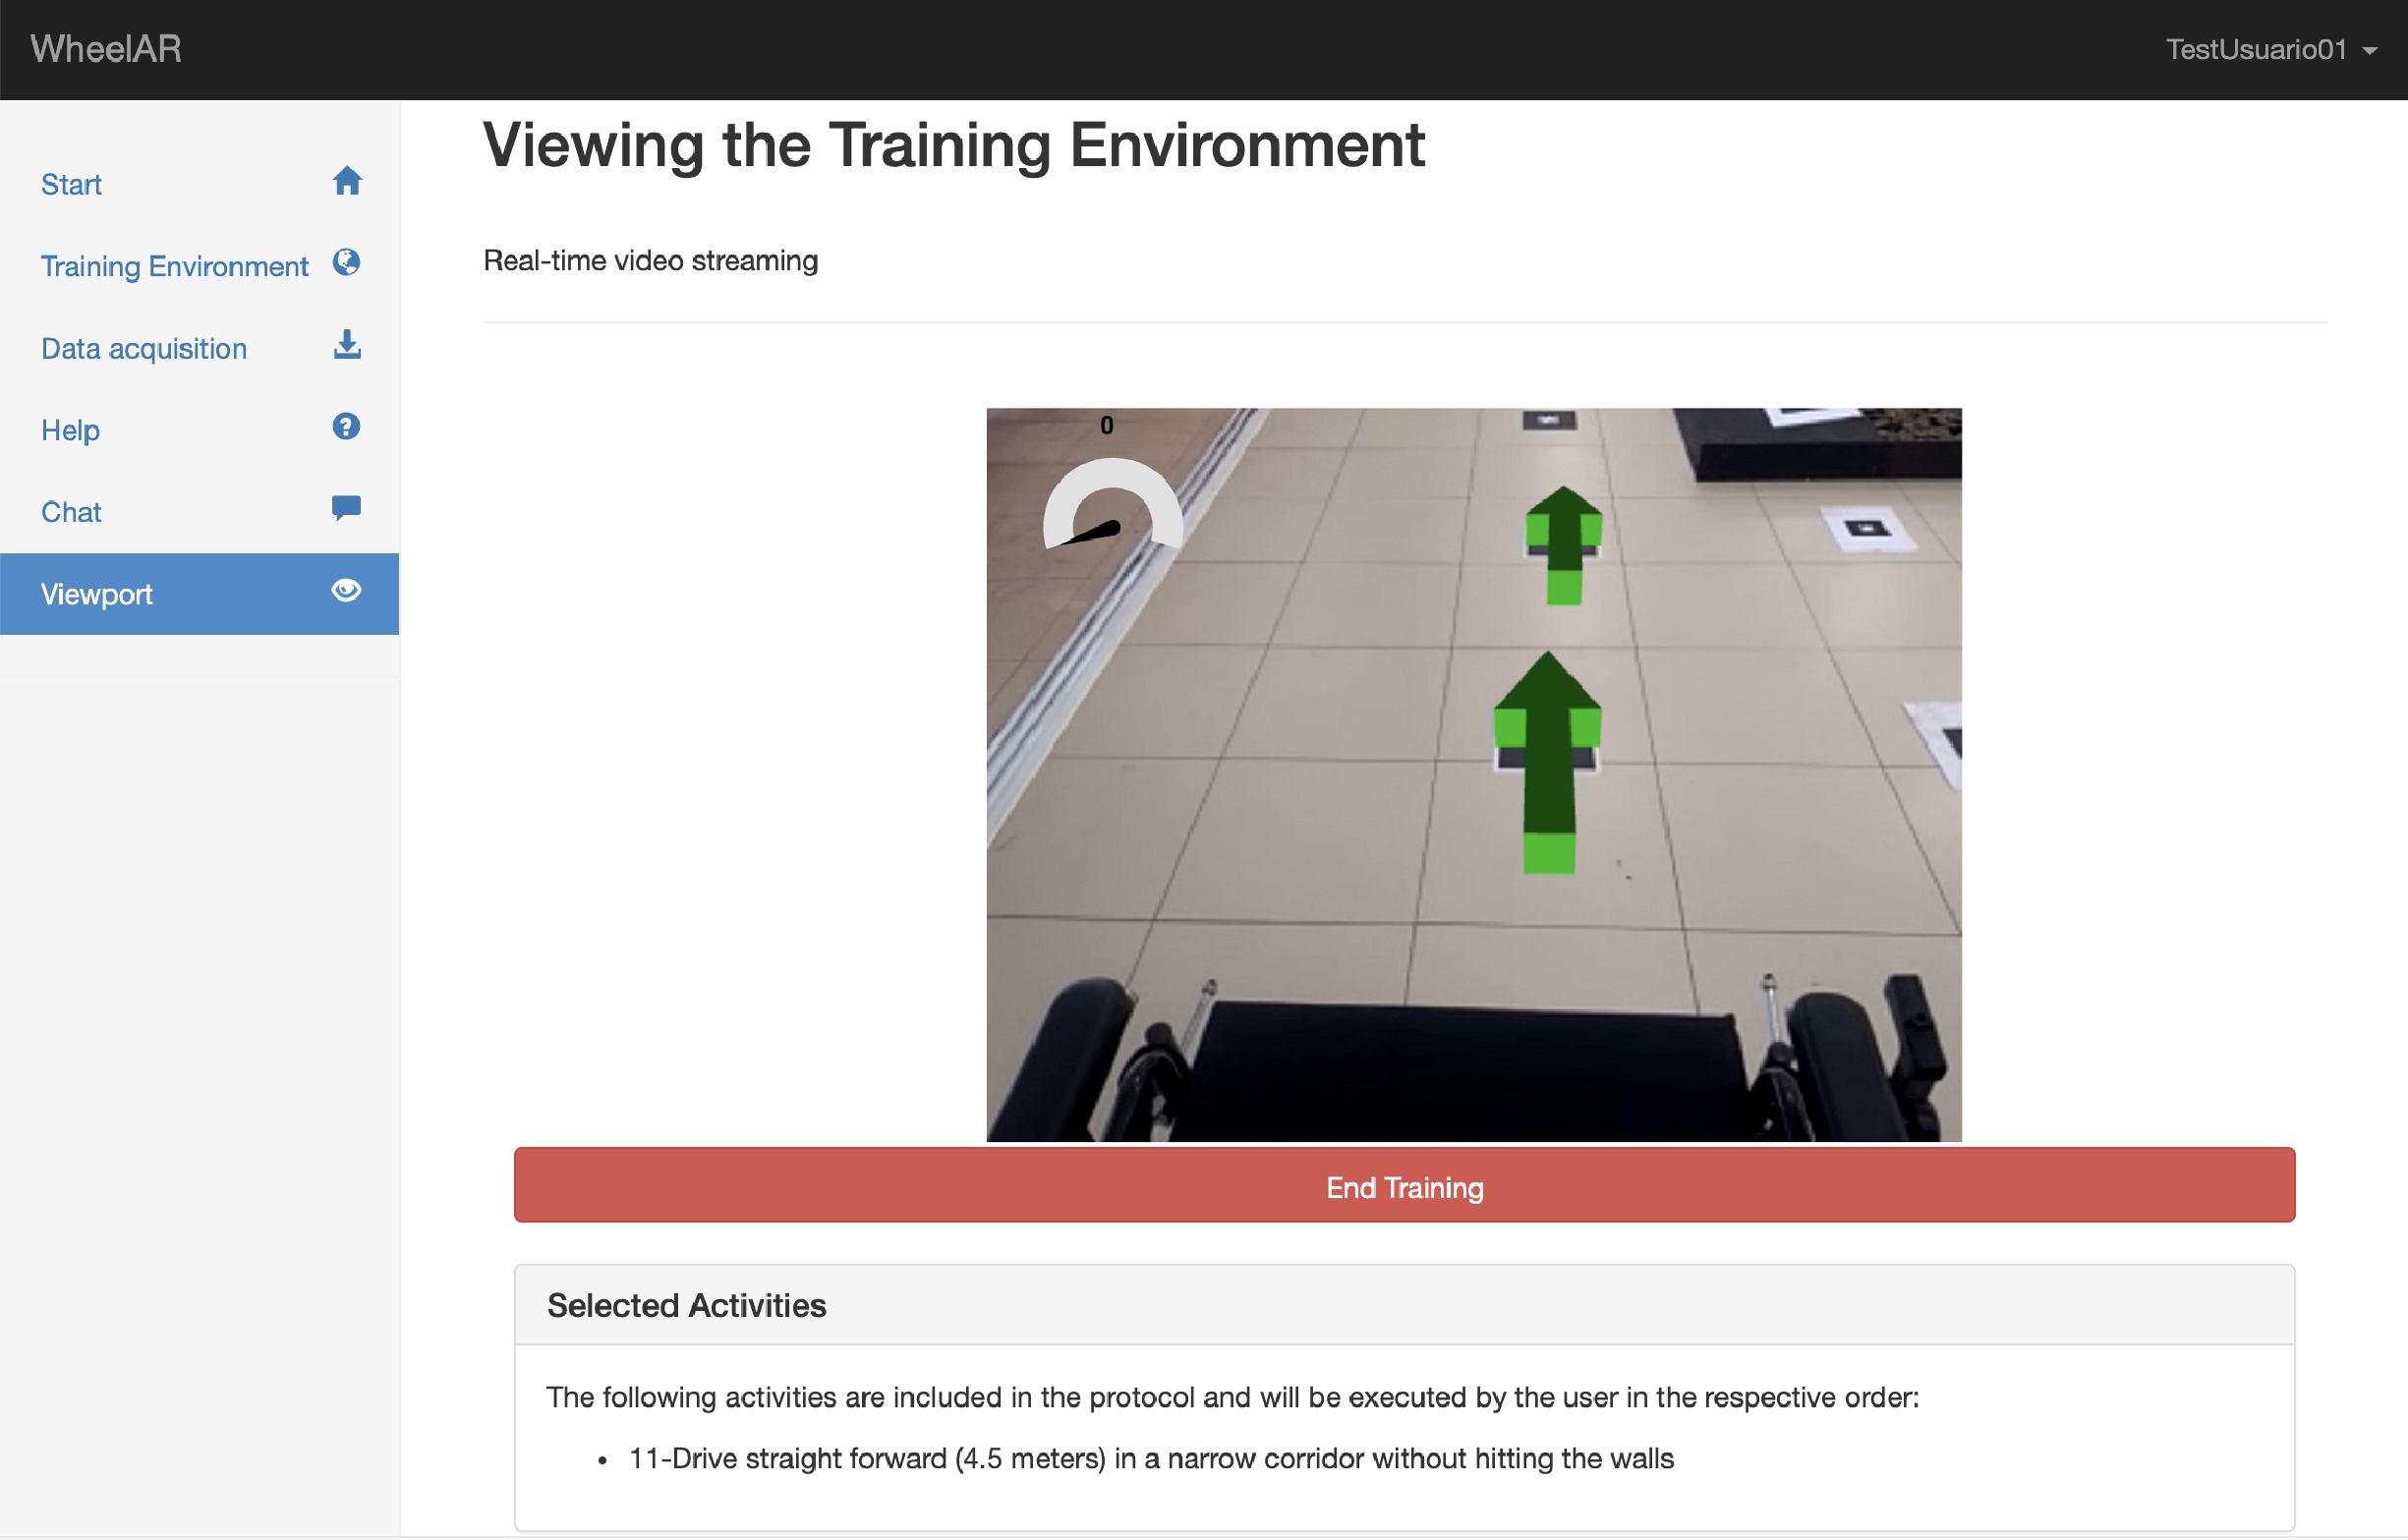
\includegraphics[width=1\linewidth]{img/cap5/tViewPortUser}
%\caption{Real-time video streaming preview page} \label{fig:tViewPortUser}
%\end{center}
%\vspace{-15pt}
%\end{figure}
%
%This view page is responsible for:  automatically connect to a shared video stream, provided from the training site; to apply  AR techniques for all received frames, to render the virtual objects over the fiducial markers; to update the PW speed value, and also, to provide a data channel using a keyboard to control PW, as needed.
%
%Again, the specific headers are charged to allow the preview of the navigation menu bar on view page load process. Going through the loading page process an HTML5 <div> tag identified as ``videos-container'' is defined into the view page body, to delimit the space that will be used for rendering graphic objects. The HTML5  <canvas> object will be stored later inside the <div> tag to update each received frame and also to render the virtual elements recognized on the AR markers. Another <canvas> HTML5 tag identified as ``speedCanvas'' is used to update a graphic speed information of the PW. The code snippet illustrates these HTML5 tags used. \newline
%
%\begin{lstlisting}[frame=single,language=HTML]  % Start your code-block
%
%<div id="videos-container" style="align:center;">
%   <span id="preview-textfield"  </span>
%   <canvas id="speedCanvas" width="150"> </canvas> </div>
%\end{lstlisting}
%
%Several JavaScript and libraries functions are imported to support some events on the front-end after the tags including process. Before starting to preview the augmented feedback from training site, the following workflow (Figure \ref{fig:ViewPortFluxogram}), is executed:
%
%\begin{figure}[!hbt]
%\begin{center}
%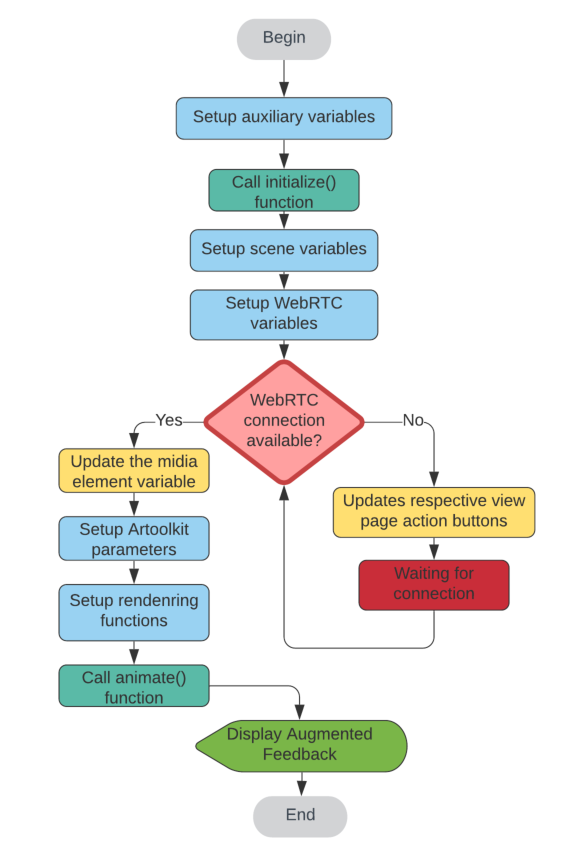
\includegraphics[width=0.5\linewidth]{img/cap5/ViewPortFluxogram}
%\caption{ViewPort Fluxogram for redering AR feedback} \label{fig:ViewPortFluxogram}
%\end{center}
%\vspace{-15pt}
%\end{figure}
%
%A main JavaScript code block is implemented to ensure that multiple updates and modifications to the content of this ``ViewPort'' dynamically occur. For this reason, in ``Setup auxiliary variables'' block, many global variables that represents different class of objects are defined and separated by classes, such as:
%\begin{itemize}
%\item 3D objects: scene, camera, renderer, mixer, clock and div\_container;
%\item ARtoolkit features: artoolkitSource, arToolkitContext and markerRoot;
%\item PW speedometer: opts, counter, gauge, taxadeAmostragem, totalTime and deltaTime; 
%\item WebRTC features: WebRTCscr and connection; and
%\item Training features: assesIDViewPort, nMarkers, ncolumn, nrows and nActivities;
%\end{itemize} 
%
%The variables belonging to 3D object class are used for any and all operations like rendering, animation and positioning of 3D primitive objects and to import elaborated objects. For that, free libraries like Three.js\footnote{https://threejs.org/}, WebGL\texttrademark\footnote {https://developer.mozilla.org/pt-BR/docs/Web/API/WebGL\_API} and glTF\texttrademark\footnote{https://www.khronos.org/gltf/} which are stored in the ``/js'' and ``js/vendor/three.js/'' folders are used.
%
%The Threex-Artoolkit\footnote{https://github.com/jeromeetienne/AR.js} is an extension of the Three.js library that handles JsArtoolkit resources and is stored in ``js/vendor/threex/''. Through three classes of objects, ArToolkitSource, ArToolkitContext and ArMarkerControls, you can easily manipulate AR. The ArToolkitSource object is responsible for tracking a marker from different sources such as a webcam, a video, or even an image. The ArToolkitContext object is the main engine and is used to deal with the position of the marker in the image source. Finally, the ArMarkerControls object, which in this case will be represented by the markerRoot variable, is responsible for positioning the content on the marker.
%
%The library Gauge.js\footnote{https://bernii.github.io/gauge.js/} is a graphic (Figure \ref{fig:speedometerPW}) object (speedometer) responsible for updating speed values and is stored in ``js/''. 
%
%\begin{figure}[!hbt]
%\begin{center}
%
\includegraphics[width=0.4\linewidth]{img/cap5/speedometer}
%\caption{PW speedometer component} \label{fig:speedometerPW}
%\end{center}
%\end{figure}
%
%The gauge and opts variables are used respectively to build the object and define its properties.
%
%WebRTC\footnote{https://github.com/muaz-khan/WebRTC-Experiment} is a framework supported by several browsers to establish the sharing of video, audio, data protocols through a browser, between different points is stored in ``js/dist/'' folder. The connection and WebRTCscr variables are used respectively to handle the connection and to establish a video and audio stream, and also, to store the remote source element identification to be used by ArtoolkitSource component.
%
%In addition to the previously mentioned variables, the ``Training features'' are essential. Among them, the most important is ``assesIDViewPort'' because it is associated with the training session requested by the user, which will be performed. Thus, all other information can be filtered, allowing virtual objects to be adequately rendered in each marker. Such information is established when creating and defining a training protocol. 
%
%The block ``Call initialize() function'' is evoked when the connection between two or more points is established considering, the basic structure for the rendering video being already ready. For this, the actions performed ``Setup scene and WebRTC variables'' are described. \newline
%
%
%\begin{lstlisting}[frame=single,language=Java]  % Start your code-block
%
%  var target = document.getElementById('speedCanvas');
%  scene = new THREE.Scene();
%  renderer = new THREE.WebGLRenderer({antialias : true, 
%     alpha : true });
%  div_container = document.getElementById("videos-container");
%  div_container.appendChild(renderer.domElement);
%  mixer = new THREE.AnimationMixer(scene);
%  clock = new THREE.Clock();
%  connection = new RTCMultiConnection();  
%  connection.socketURL = 
%     'https://rtcmulticonnection.herokuapp.com:443/';
%  connection.session = { audio : false, 
%      video : true, oneway : true };
%  connection.videosContainer = document.getElementById
%      ('videos-container');
%  window.addEventListener('keydown', onKeyDown, false);
%  
%//Call stream available function 
%  connection.onstream = function(event) {
%     webRTCsrc = event.mediaElement; \\updating mediaURL
%\end{lstlisting}
%
%Among these block actions, the canvas object, in which the speedometer will be displayed, is assigned to the ``target'' variable. Next, the ``scene'' variable is initialized to be responsible for receiving other objects to be rendered. Additional objects, such as light (ambient and directional) and a camera incorporated into the ``scene'' are defined. However, properties definition were omitted, but have been established in this code. 
%
%The ``renderer'' object is defined because it is from the properties, every frame information received is processed and updated. It's properties definitions such as size, lighting and position have also been omitted, but they have been implemented. 
%
%The <div> tag identified as ``videos-container'' is assigned to the ``div\_container'' variable, because it is used as a rendering objects container. Since our idea is to work with dynamic 3D and not only static objects, a ``mixer'' variable is initialized with the previous ``scene'' object created for animating objects. For this reason, a ``clock'' and also `` deltaTime and totalTime'' are initialized, in order to help in rendering time process control.
%
%As every rendering process requires a video stream, and in our case, this stream is remotely shared, the ``connection'' variable is initialized as an object of the RTCMultiConnection class. Thus, a sharing URL server is defined to handle it. Also, it is necessary to define what is this flow property, whether it will have video, audio, etc. 
%
%So, before calling the ``onstream'' function, responsible for handling these connections, a keyboard event listener (handled by ``js/keyBoard.js'' file ) is associated with the page body to allow, the keyboard can also be used as a PW control interface. 
%
%After calling the, ``onstream'' function, the processes are paused, until receiving a confirmation message that the stream has started. For this, the WebSockets API\footnote{https://developer.mozilla.org/en-US/docs/Web/API/WebSockets\_API} is used to establish communication channels between different points. In the meantime, the action buttons are updated based on the user profile, in addition to the activities list to be performed. The only action button for this profile is ``End training'' managed by ``ServletMain''. It updates on the database, information such as the finishing training time, and the user's status: online, freeing the use of the training site, redirecting him to the user view page.
%
%However, after receiving the message, first, the variable ``webRTCsrc'' is updated with the remote media object information. Then, all the actions by the blocks ``Setup ArtoolKit and Rendering functions'' are performed. 
%
%There are three configurations to be made in Artoolkit: the ArToolkitSource, ArToolkitContext and ArMarkerControls. The ``ArToolkitSource'' variable is initialized according to the first line of code in the command block. As seen, the ``webcam'' is defined as the streaming source. However, an adaptation was performed in the ``js/vendor/threex/threex-artoolkitsource.js'' library because the physical device ( present on the notebook or computer) address is automatically defined. In our case, this source is remote, for this reason, the ``ARjs.Source.prototype.\_initSourceWebcam'' function was modified to receive as a source, the object saved by the variable ``webRTCsrc''. Thus, the ``arToolkitSource.onResize()'' function can be performed. The stream renderer object source is no longer null, and then the arToolkitContext information is updated. Thus, the arToolkitSource ``onReady()'' function initializes the PW speedometer (gauge) and add another event listener, associated with the window resize actions.\newline
%
%\begin{lstlisting}[frame=single,language=Java]  % Start your code-block
%
%arToolkitSource = new THREEx.ArToolkitSource({sourceType : 
%  'webcam',});
%
%function onResize() {
%  arToolkitSource.onResize()
%  arToolkitSource.copySizeTo(renderer.domElement)
%  if (arToolkitContext.arController !== null) {
%      arToolkitSource.copySizeTo(arToolkitContext.arController.
%      canvas) }}
%
%arToolkitSource.init(function onReady() {
%  onResize()
%  gauge = new Gauge(target).setOptions(opts); // create gauge!
%  });
%window.addEventListener('resize', function() { onResize()});
%
%\end{lstlisting}
%
%Then, the next step is to initialize the variable ``arToolkitContext''. As described in the code below, the parameters ``camera\_para.dat'' file are loaded and the image detection mode is defined. Finished the loading process, these parameters are duly copied to the artoolkitContext camera. \newline
%
%\begin{lstlisting}[frame=single,language=Java]  % Start your code-block
%
%  arToolkitContext = new THREEx.ArToolkitContext({
%    cameraParametersUrl : 'data/data/camera_para.dat',
%    detectionMode : 'mono'});
%  // copy projection matrix to camera when init is complete
%  arToolkitContext.init(function onCompleted() {
%    camera.projectionMatrix.copy(arToolkitContext.
%    getProjectionMatrix()); });
%\end{lstlisting}
%
%The last configuration to be performed in Artoolkit is ArMarkerControls. For this, it is necessary to generate the patterns files (.patt) who defines each fiducial AR marker feature and the 3D object (.glTF) to be loaded. Based on the size of the AR matrix, defined in Section \ref{sec:createProtocol}, or by the product between the variables (``nrows'' and ``ncolumns'') it is possible to know the amount of markers needed. To generate  AR markers image, based on the Artoolkit standard, the Python AR markers\footnote{https://github.com/MomsFriendlyRobotCompany/ar\_markers} library was used. After exporting all images, it is necessary to generate the patterns files to be used by ArMarkerControls. These files were generated using the AR.js Marker training\footnote{https://jeromeetienne.github.io/AR.js/three.js/examples/marker-training/examples/generator.html} library displayed by Figure \ref{fig:jeromeetienneAR-Maker}. From the ``upload'' button the an image file is loaded and then from the button ``Download Marker'' the pattern file exported. All generated files are stored in the ``data/data/'' folder.
%
%\begin{figure}[!hbt]
%\begin{center}
%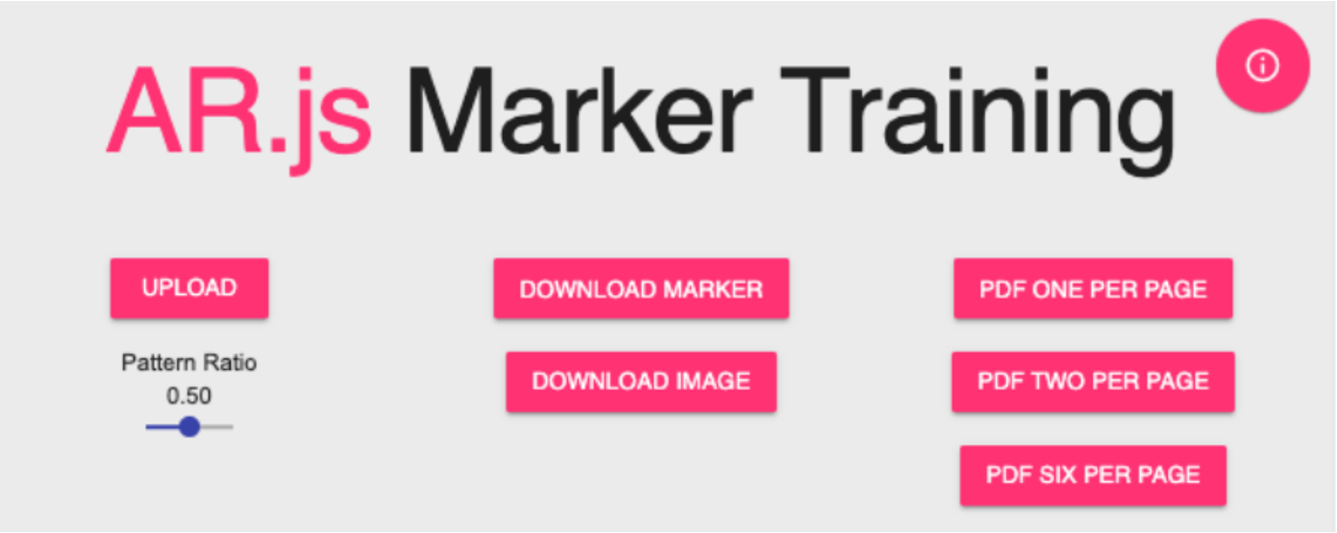
\includegraphics[width=1\linewidth]{img/cap5/jeromeetienneAR-Maker}
%\caption{AR.js Marker Training Maker page} \label{fig:jeromeetienneAR-Maker}
%\end{center}
%\end{figure}
%
%Therefore, the next step is to generate a string vector, where each element is the name of each pattern file, in an example, pattern-00 as exemplified by the code extracted. \newline
%
%
%\begin{lstlisting}[frame=single,language=Java]  % Start your code-block
%
%  var patternArray = [];
%  var nMarkerPatterns = 0;
%  for (var nr = 0; nr < nrows; nr++) {
%    for (var nc = 0; nc < ncolumn; nc++) {
%      if (nMarkerPatterns < 10)
%	 patternArray.push("pattern-0" + nMarkerPatterns);
%      else
%	 patternArray.push("pattern-" + nMarkerPatterns);
%    nMarkerPatterns++;
%    }
%  }
%\end{lstlisting}
%
%
%The 3D objects were generated using Blender$^{\textregistered}$. After animating and drawing, the following export process must be performed. First, a 3D model is selected (Figure \ref{fig:3dModel-Blender}), then click on the menu ``File> Export> glTF 2.0''. In the following dialog box (Figure \ref{fig:glTFExportSettings}), select the highlighted format (glTF Separated + textures). In the Textures field, inform the path where the texture will be saved, for example, ``myModels/textures''. Check the ``selected object'' option and leave the animation options checked, as ilustrated by (Figure \ref{fig:glTFExportSettings}). If the Blender version is prior to 2.8, it is necessary to proceed with the plugin\footnote{https://github.com/KhronosGroup/glTF-Blender-IO} installation. Finally, press ``Export glTF 2.0'' button and select the folder where the models will be stored. In this project, the glTF models are stored in ``models/gltf'' folder.
%
%\begin{figure}[!htbp]
%\center
%\begin{minipage}{0.495\linewidth}
%\center
%\captionsetup{justification=centering,margin=0cm,font=small}
%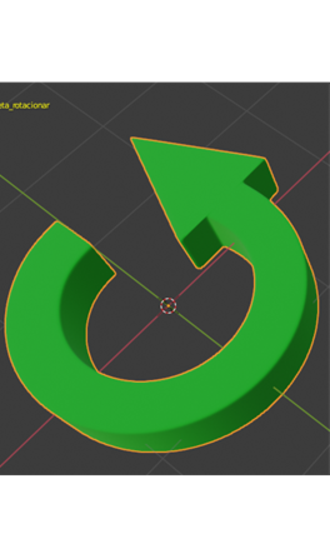
\includegraphics[width=1\linewidth]{img/cap5/3dModel-Blender}
%\caption{3D animated Blender Model} \label{fig:3dModel-Blender}
%\end{minipage}
%\begin{minipage}{0.495\linewidth}
%\center
%\captionsetup{justification=centering,margin=0cm,font=small}
%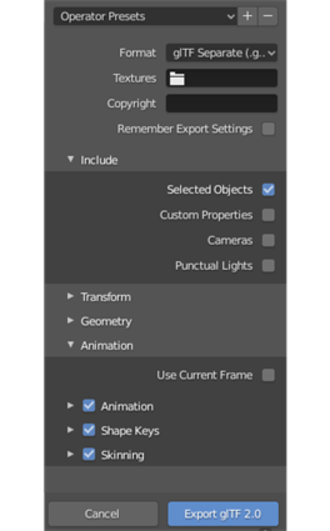
\includegraphics[width=1\linewidth]{img/cap5/glTFExportSettings}
%\caption{glTF Export Settings} \label{fig:glTFExportSettings}
%\end{minipage}
%\end{figure}
%
%To complete the process, each pattern file has to be associated with the respective model and adjust its properties. The following snippet code demonstrates these implemented steps. The ``nMarkers'' variable is a ``string'' containing the 3D objects name, associated by the therapist in each AR matrix position.  Each element of the ``ObjectToRender '' vector is filled with these split names, whose size equals to the variable ``nMarkerPatterns''. Thus, through the implemented repeating structure, it is possible to assign the ``markerControls'' variable to each marker pattern to the controller. Then, through the GLTFLoader library, stored in the ``js/'' folder, it is possible to read each 3D model file. For those AR matrix positions, where no objects were associated, the assigned value is ``none''. Therefore, before calling the ``loadAnimation()'' function, it is checked of the ``ObjectToRender'' vector element is equal to ``none''. So, no object is rendered in that marker. On the other hand, it is verified whether the 3D model is static or animated. If it is an animation, the 3D model is linked to a ``mixer'' object, with its properties duly changed, allowing them to be animated in the future. Finally, the object is added to the scene ``markerRoot'' list elements. \newline
%
%\begin{lstlisting}[frame=single,language=Java]  % Start your code-block
%
%  var ObjectToRender = [];
%  ObjectToRender = nMarkers.split(';');
%  for (let i = 0; i < nMarkerPatterns; i++) {
%    scene.add(markerRoot);
%    let markerControls = new THREEx.ArMarkerControls(
%       arToolkitContext, markerRoot, {type : 'pattern',
%       patternUrl : "data/data/" + patternArray[i]+ ".patt",});
%     var loader = new THREE.GLTFLoader();
%     var path_model = "models/gltf/";
%     if (ObjectToRender[i] != "none") { 
%        loadAnimation();
%     }
%  function loadAnimation() {
%    var filename = path_model + ObjectToRender[i] + ".gltf";
%    loader.load(filename, function(gltf) { 
%    if (gltf.animations[0] != null) {
%       mixer = new THREE.AnimationMixer(modelo);
%       mixer.timeScale = 1;
%       mixer.clipAction(gltf.animations[0]).play();
%      }
%      markerRoot.add(modelo);
%      }, undefined, function(e) {
%      console.error(e);}); 
%  } ;
%  } //fim for
%\end{lstlisting}
%
%Once, having configured all the components responsible for generating the AR feedback from the training site, it is necessary to define the rendering functions. From the code snippet below, the ``update()'' function is responsible for updating virtual objects over each fiducial AR marker. \newline 
%
%\begin{lstlisting}[frame=single,language=Java]  % Start your code-block
%
%  function update() {
%    // update artoolkit on every frame
%    if (arToolkitSource != undefined && arToolkitSource.ready 
%       !== false)
%       arToolkitContext.update(arToolkitSource.domElement); }
%\end{lstlisting}
%
%
%Next, the ``render()'' function, updates the runtime parameters of the 3D models, the scene objects, camera and speedometer. Every 10 fps the ``ajaxSyncRequest()'' function make a GET request to `` ServletSpeedPW '' that retrieves from the assessTH table the current PW speed value to update the speedometer. \newline 
%
%\begin{lstlisting}[frame=single,language=Java]  % Start your code-block
%
%  function render() {
%    mixer.update(clock.getDelta());
%    renderer.render(scene, camera);
%    if (gauge != undefined) {
%      if(taxaDeAmostragem==10){
%	ajaxSyncRequest(assesIDViewPort);
%	taxaDeAmostragem=0;
%	gauge.setTextField(document.getElementById(preview-
%        textfield));			
%	gauge.set(counter);
%	}else{
%	   taxaDeAmostragem++;  } } }
%
%\end{lstlisting}
%
%Thus, the function ``animate()'' is evoked by a received frame event, afford the AR feedback as shown in Figure \ref{fig:tViewPortUser}. However, if the connection is closed by the user, some inconsistency, or due to quality restrictions of the WebRTC itself,  the 3D rendering objects are automatically hidden and disabled. \newline
%
%\begin{lstlisting}[frame=single,language=Java]  % Start your code-block
%
%     function animate() {
%     requestAnimationFrame(animate);
%     deltaTime = clock.getDelta();
%     totalTime += deltaTime;
%     update();
%     render(); }
%\end{lstlisting}
%
%
%\subsubsection{Data acquisition} 
%
%
%Since a web browser is a sandbox application, to issue commands inputs to a remote PW, the user has to download the cross-platform Java\texttrademark  \hspace{4pt}application shown in Figure \ref{fig:dataAcquisition01} and \ref{fig:dataAcquisition02}. From this application, a data connection with the ``ServletCommand'' is established. 
%
%\begin{figure}[!htbp]
%\center
%\begin{minipage}{0.45\linewidth}
%\center
%\captionsetup{justification=centering,margin=0.5cm,font=small}
%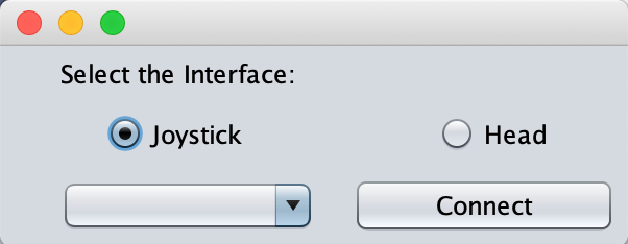
\includegraphics[width=1\linewidth]{img/cap5/dataAcquisition01}
%\caption{Starting dataflow} \label{fig:dataAcquisition01}
%\end{minipage}
%\begin{minipage}{0.45\linewidth}
%\center
%\captionsetup{justification=centering,margin=0cm,font=small}
%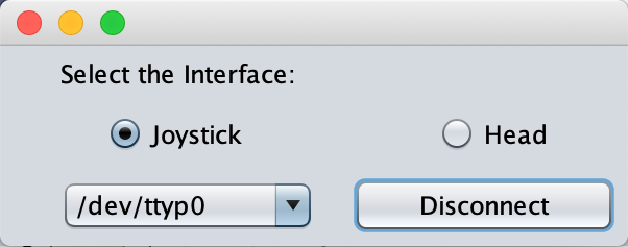
\includegraphics[width=1\linewidth]{img/cap5/dataAcquisition02}
%\caption{Close dataflow} \label{fig:dataAcquisition02}
%\end{minipage}
%\end{figure}
%
%This servlet is responsible for forwarding all control input to the training site. However, when a keyboard is used as an interface control, this application is not requested, because the browser recognizes the keyboard as basic input. 
%
%The application implementation core is based on the Java Interfaces (shown in the code snippet) concept. \newline
%
%\begin{lstlisting}[frame=single,language=Java]  % Start your code-block
%
%public interface deviceConnector {
%  public void deviceSensor();
%  public void dataProcessor();
%  public void forwardData();  }
%\end{lstlisting}
%
%Each control interface (EMG, EEG, Eye-tracking, and others) has the same control actions, although the data is different. The UML Class Diagram shown in Figure \ref{fig:deviceData} illustrates it.
%
%\begin{figure}[!hbt]
%\begin{center}
%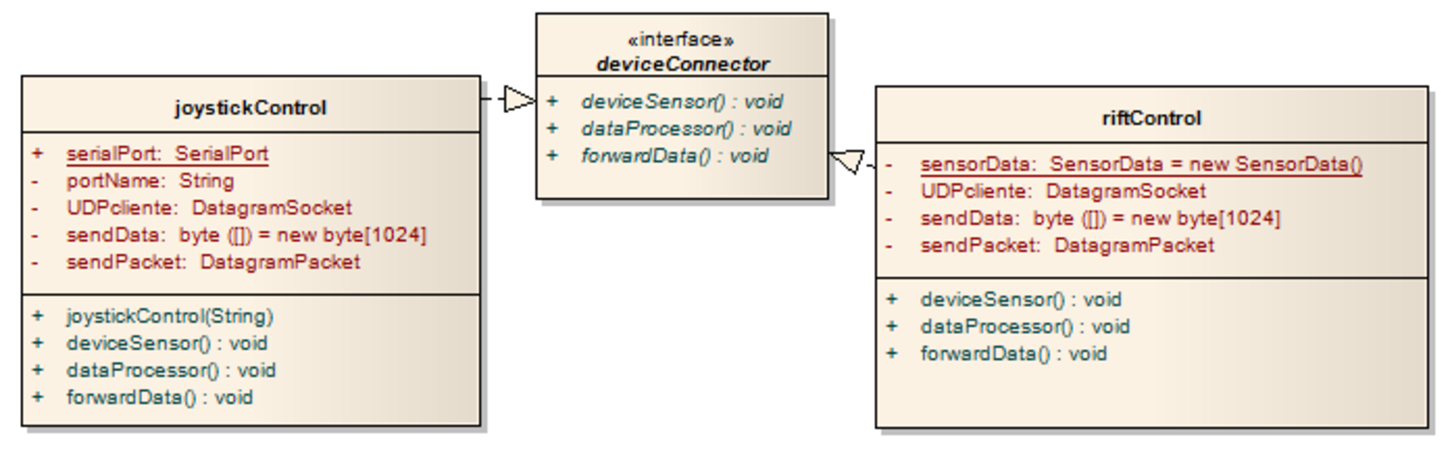
\includegraphics[width=1\linewidth]{img/cap5/deviceData}
%\caption{Class Diagram for handling with different class of data} \label{fig:deviceData}
%\end{center}
%\end{figure}
%
%
%As a concept proof, it was used the joystick and head movements control interfaces. Since, to form the control commands using the joystick, voltage values are analyzed and for the head movements values (yaw, pitch and row). Thus, to any interface control used the following workflow will be followed:
%
%\begin{enumerate}
%\item deviceSensor: it is responsible for recognizing each interface controle conected in a computer or notebook; 
%\item dataProcessor: it is responsible for collection and proceeds with data processing. For each signal, have to make some pre-processing procedures to let this data ready to be classified. After, in the agreement of for each class of signal recognized it belongs of one this command protocol defined: 5 - PW stopped; 1 - PW turn right; 2 - PW turn left; 3 - PW move backward; 4 - PW move forward;
%\item forwardData: using the HTTP POST method\footnote{https://developer.mozilla.org/en-US/docs/Web/HTTP/Methods/POST}, as described by the code block, a single string carrying the numeric value is sent to the ``ServletCommand''. After the therapist releasing, this servlet proceeds with all metrics measuring in or order to provide the relevant data for the therapist training session evaluation.
%\end{enumerate}
%
%
%\begin{lstlisting}[frame=single,language=Java]  % Start your code-block
%
%String url = "http://server:8080/webApp/command/"+aux;
%HttpClient client = new DefaultHttpClient();
%HttpPost post=null;
%post = new HttpPost(url);
%post.setHeader("User-Agent", "Mozilla/5.0");
%HttpResponse response = client.execute(post);
%\end{lstlisting}
%
%
%To start the data-flow, the user has to select an option. If it is ``joystick''  then select the port and then press the button ``Connect''  or ``Disconnect'' to close data-flow and application. 
%
%
%\subsection{Therapist session}
%
%
%The following UC actions, described in Figure \ref{fig:therapistCases}, were implemented to support the therapist's actions in the telerehabilitation process of PW user's. 
%
%\subsubsection{User register}
%
%The view page presented by Figure \ref{fig:tUserRegister}  (stored as register.jsp) illustrates the second UC implementation performed by the therapist. 
%
%\begin{figure}[!hbt]
%\begin{center}
%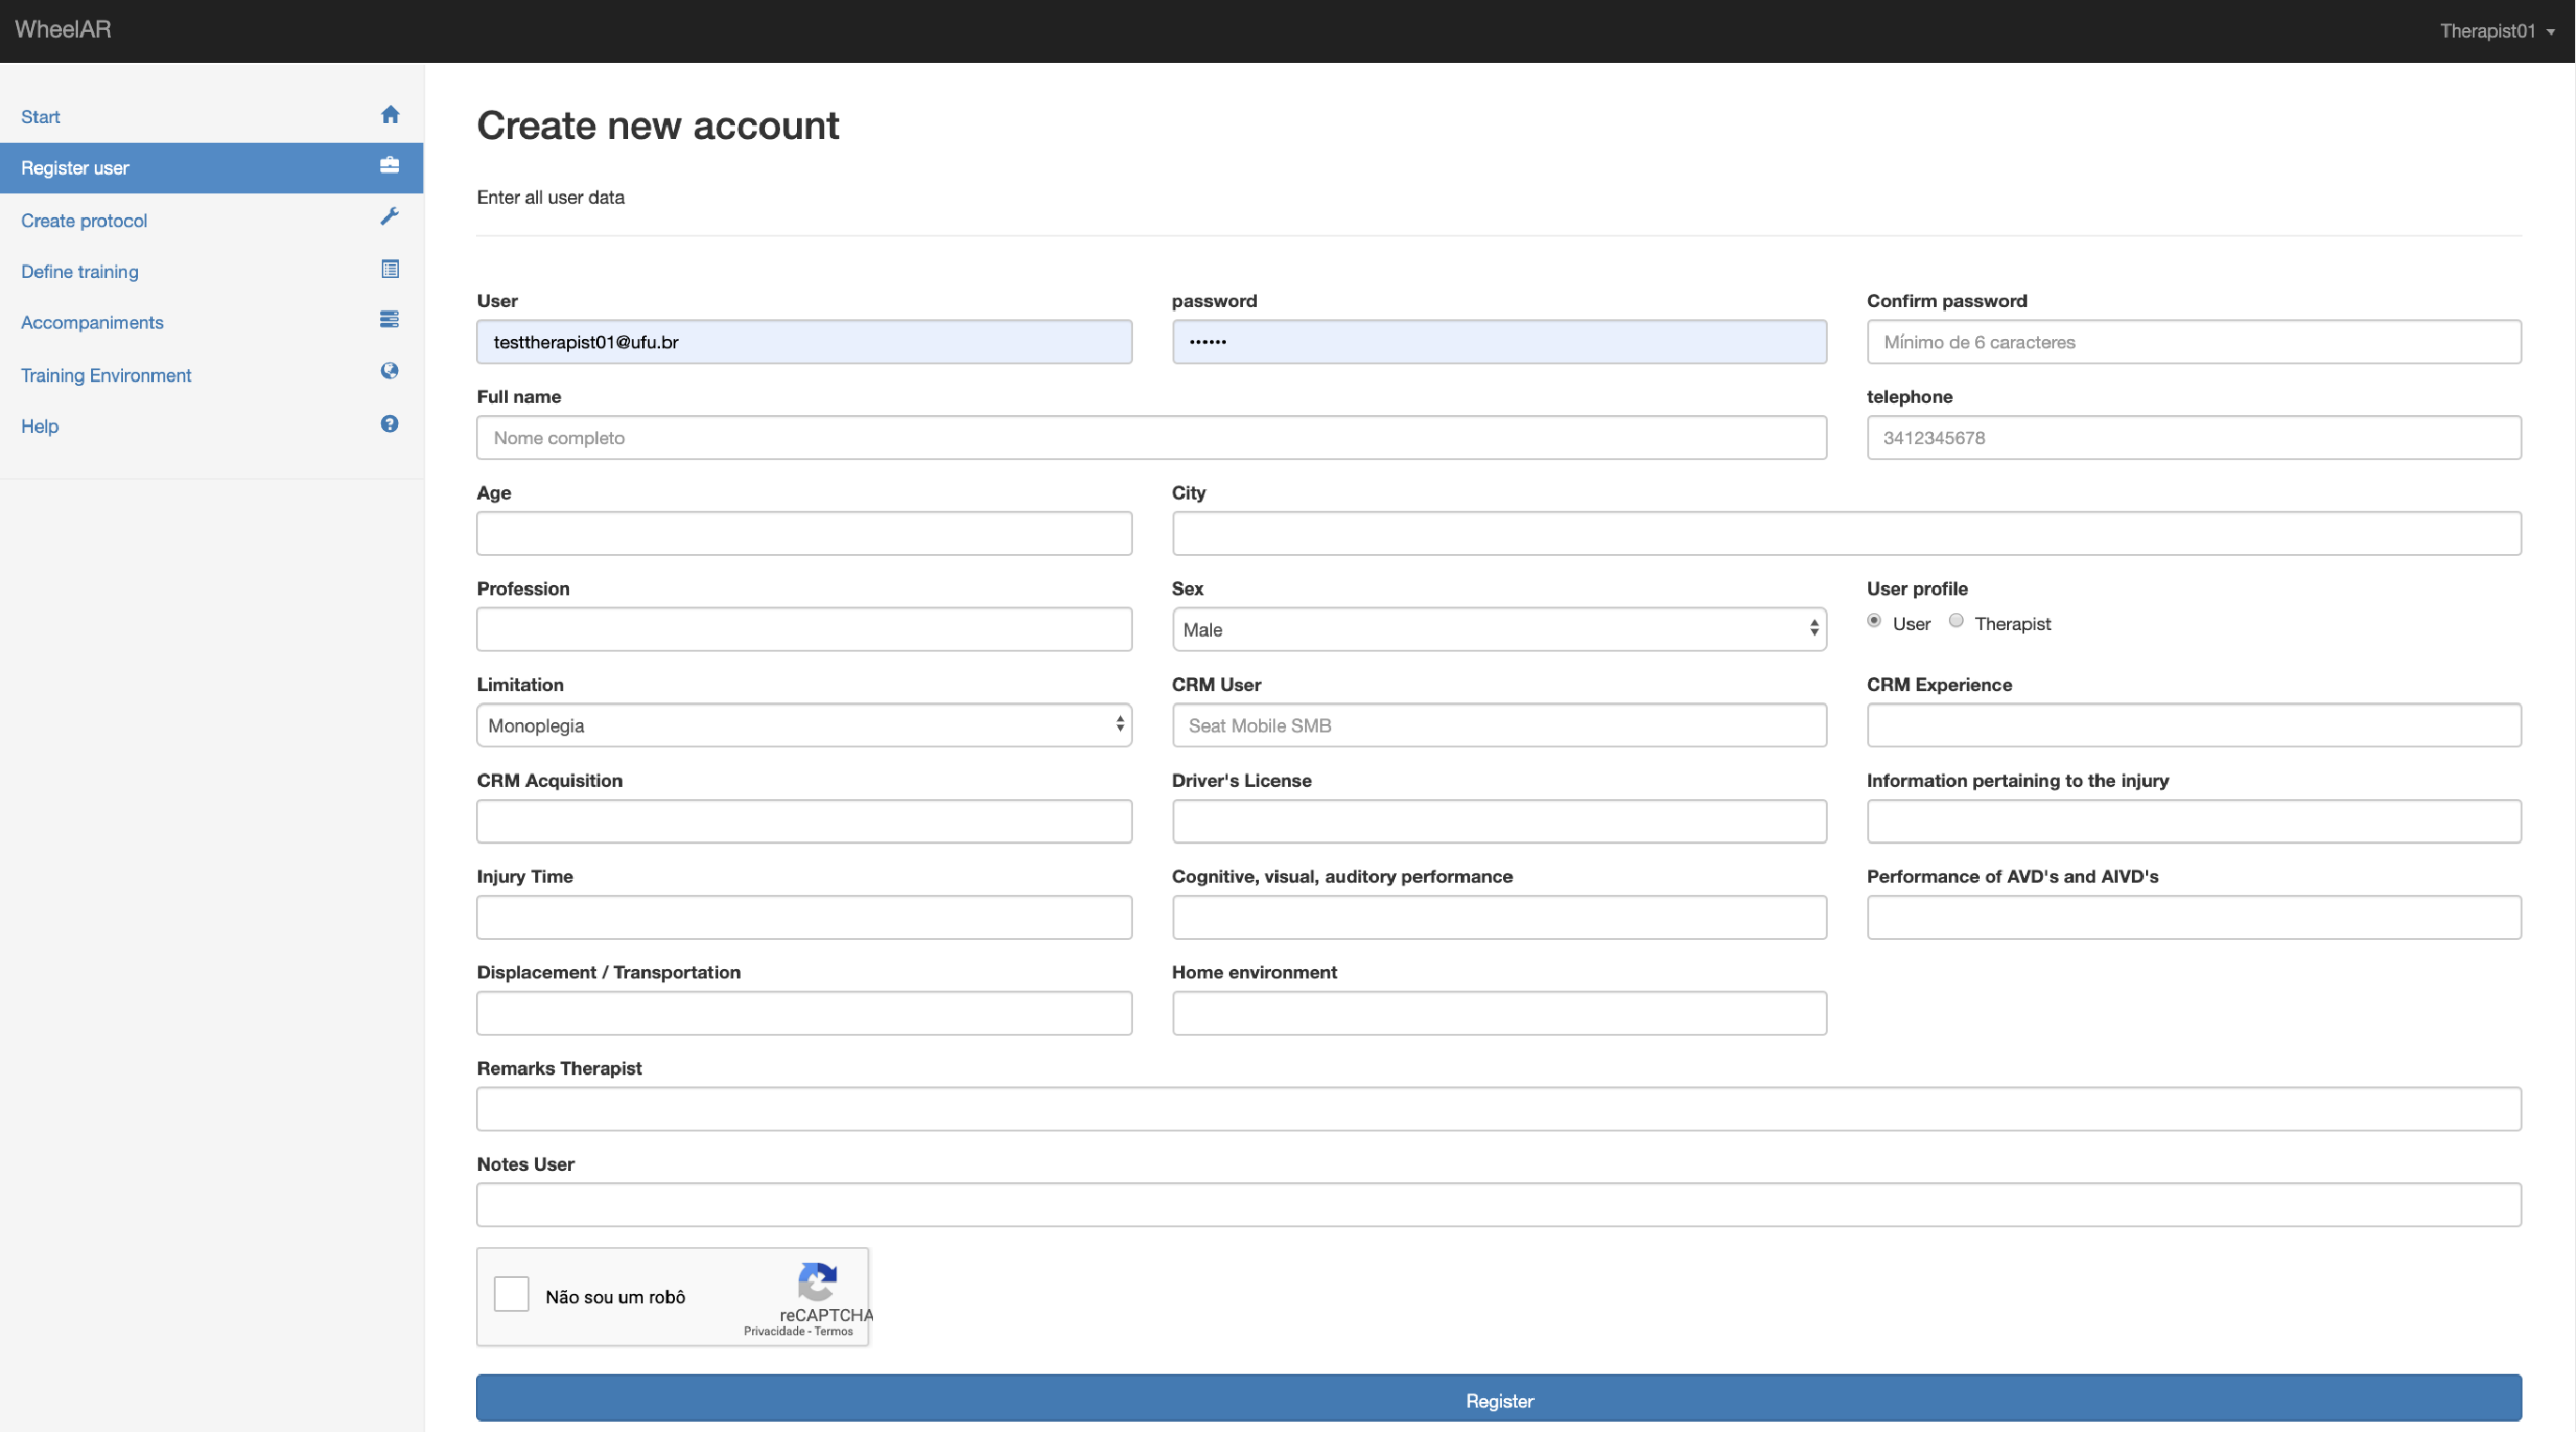
\includegraphics[width=1\linewidth]{img/cap5/tUserRegister}
%\caption{Register a new user page} \label{fig:tUserRegister}
%\vspace{-10pt}
%\end{center}
%\end{figure}
%
%According to the selected profile option, a JavaScript method action ``showForm'' is triggered by a radio button event. It updates field information to be stored in the database. Before submitting the  ``Register'' action to the ``ServletRegister'' controller, it's necessary to validate the captcha, where the ``VerifyRecaptcha'' controller is responsible. After, a ``Register'' button action is submitted to the respective controller, which implements the actions described in the SD action shown in Figure \ref{fig:UMLSD-TherapistWebCase02}.  The impairments list is retrieved from the database using the following embedded Java code on .jsp file:
%\newline
%\begin{lstlisting}[frame=single,language=Java]  % Start your code-block
%
%rs = st.executeQuery(select * from impairmentTh order by 
%impairmentID);
% while (rs.next()) {
%  out.print(<option value= + rs.getString("impairmentID") + >);
%  String[] listDescript = rs.getString("description").split(":");
%  out.print(listDescript[0]);
%  out.println("</option>");}
%\end{lstlisting}
%
%
%\subsubsection{Create protocol}
%\label{sec:createProtocol}
%
%Figure \ref{fig:createProtocol01} and \ref{fig:createProtocol02} represent the view page (stored as criar\_protocolo.jsp) that  illustrates the implementation of the third UC performed by the therapist. 
%
%When ``Create protocol'' action is select into menu, different data are retrieved, such as activities and image lists to promote the PMRT adaptation actions implementation. A user guide, that describes how to proceed with ``Create protocol'' SD action, is shown in Appendix \ref{sec:appCreateProcotol}.
%
%\begin{figure}[!hbt]
%\begin{center}
%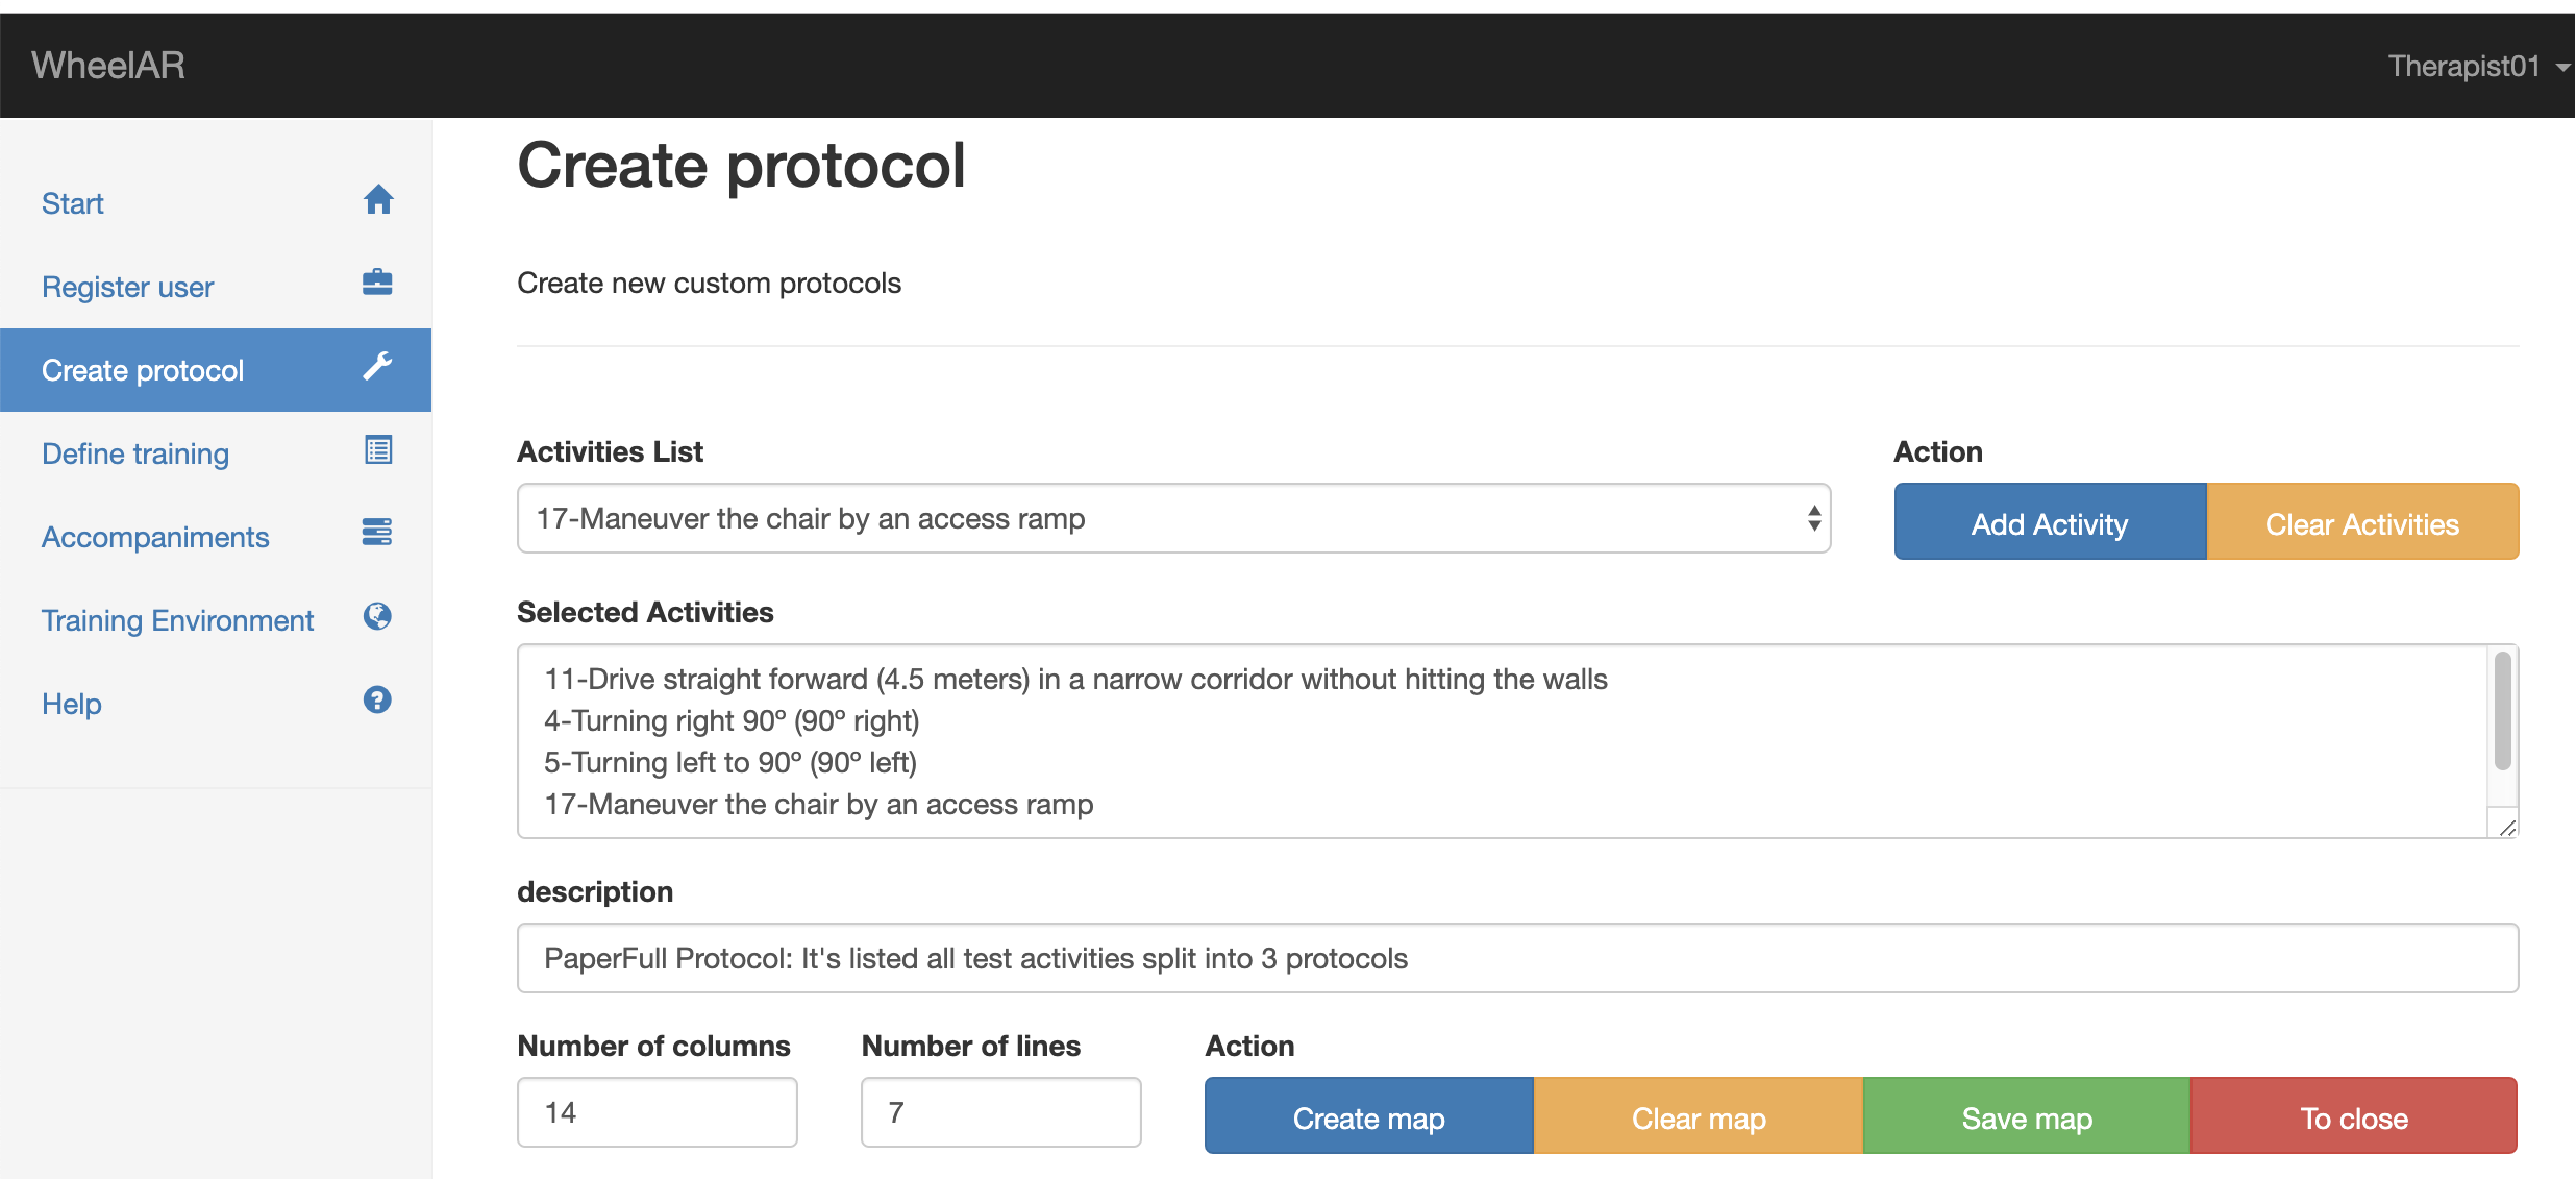
\includegraphics[width=1\linewidth]{img/cap5/tCreateProtocol01}
%\caption{Defining the activities for each protocol} \label{fig:createProtocol01}
%\end{center}
%\vspace{-10pt}
%\end{figure}
%
%\begin{figure}[!hbt]
%\begin{center}
%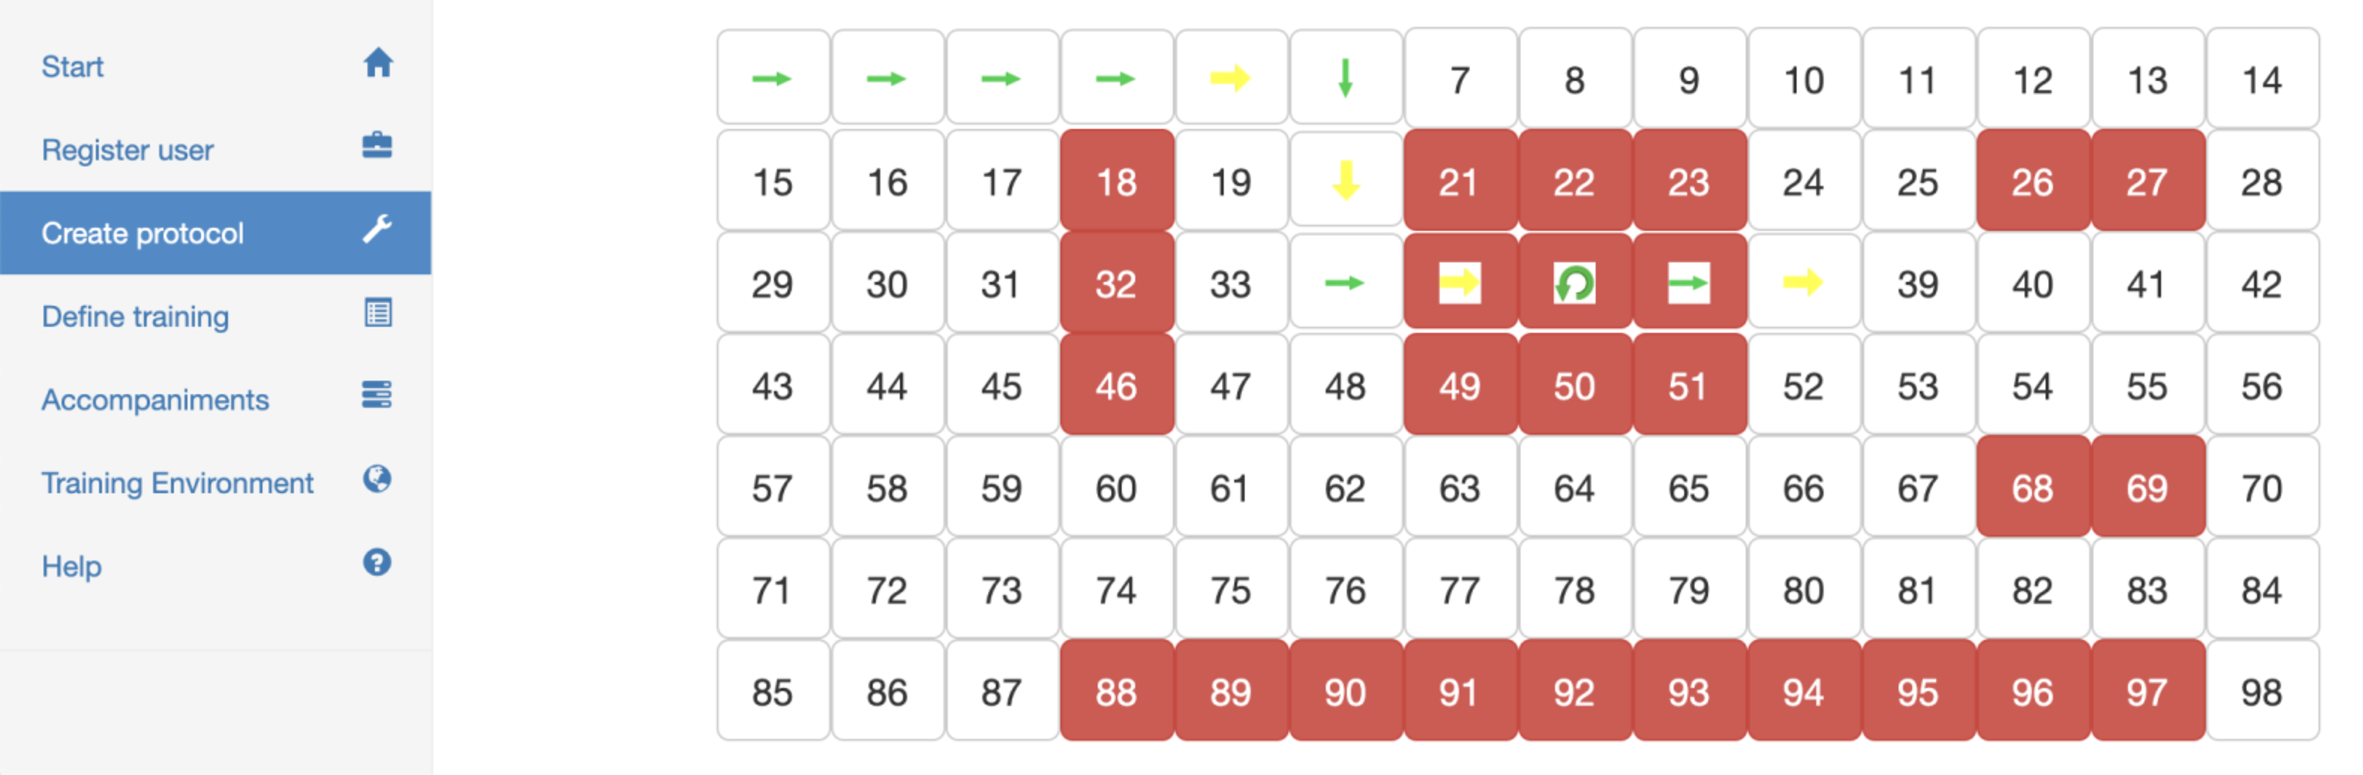
\includegraphics[width=1\linewidth]{img/cap5/tCreateProtocol02}
%\caption{Create a training activities and protocol map example} \label{fig:createProtocol02}
%\end{center}
%\vspace{-10pt}
%\end{figure}
%
%From the headerLogged.jsp file, stored in ``inc'' folder, loaded every time that's the user has logged into the system, many JavaScript files are included in the view pages. The ``matrixAR.js'' and ``formProtocol.js'' stored in ``js'' folder are very important to the ``Add and Clear Activity'' and to ``Create and Clear map'' actions. The code imported from matrixAR.js is a function example.
%\newline
%\begin{lstlisting}[frame=single,language=Java]  % Start your code-block
%
%function addAtividade() {
%  var conteudo = document.getElementById('listActivities').value;
%  var atividade =document.getElementById('activityID').options
%     [document.getElementById("activityID").selectedIndex].text;
%  document.getElementById('listActivities').value = conteudo + 
%     atividade +"\n"; }
%\end{lstlisting}
%
%The ``addAtividade and clearAtividades'' onclick event methods from ``matrixAR.js'', are inherited on ``Add and Clear Activity'' buttons. Thus, is possible update information on ``Selected activities'' field (Figure \ref{fig:createProtocol01}). Also, the ``adicionaLinha and removeLinha'' onclick event methods from ``matrixAR.js'', are inherited on ``Create and Clear map'' buttons allowing to add or remove an empty AR matrix buttons (Figure \ref{fig:createProtocol02}). Red buttons shown in the AR matrix represent physical obstacles present in the training site. 
%
%As mentioned before, an image list from folder ``img'' is created from an embedded Java code block on ``create\_protocolo.jsp'' file and save on the user session. The following event button methods (selectModel, onSubmit) are incorporated into each AR matrix button stored in ``formProtocol.js'' file to create ``Select model'' dialog, which use the image list stored in user session. 
%
%\begin{figure}[!hbt]
%\begin{center}
%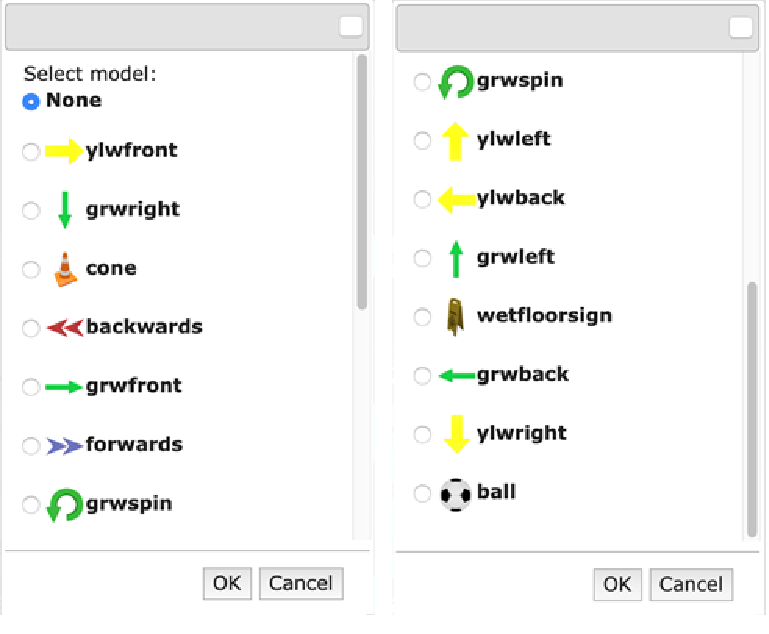
\includegraphics[width=0.6\linewidth]{img/cap5/virtualObjects}
%\caption{Virtual objects (animated/statics) list} \label{fig:virtualObjects}
%\end{center}
%\end{figure}
%
%Then, the therapist is able to define the virtual objects that can be used as guidance or avoidance and also can be static or animated, a protocol example is presented in Figure \ref{fig:createProtocol02}. Thus, it is possible to even in a controlled environment to have a non-structural activity where the user has to decide what he has to do in front of an unexpected event.
%
%The  ``Save map'' button action is handled by ``ServletMain'' used to record a new protocol in the protocolTH (Figure \ref{fig:tablesDiagram}) table, with the number of tasks that will be performed based on the map created by the therapist. The yellow arrows mark the end and the beginning of a new activity, while the green ones are used to guide the user during the protocol execution. The button  ``To close'' is used to exit the system. This Servlet is responsible for handling many different requests from different views. To distinct each request, all button event is filtered to ensure each SD action be performed appropriately, as described by the following snippet code.\newline
%
%
%\begin{lstlisting}[frame=single,language=Java]  % Start your code-block
%
%protected void doPost(HttpServletRequest request, 
%HttpServletResponse response) throws ServletException, 
%IOException {
%  userButton = request.getParameter("userButton");
%  //Verificacao de eventos para registro do survey
%  if (userButton.equals("registrar"))
%     buttonRegistrar(request, response);
%  //Acao selecionar paciente da pagina: acompanhamentos
%  if (userButton.equals("selecionarPaciente"))
%      buttonSelecionarPaciente(request, response);
%\end{lstlisting}
%
%\subsubsection{Define protocol}
%\label{sec:definedProtocol}
%
%Figure \ref{fig:tDefineProtocol01} shown the view page (stored as definir\_treinamento.jsp) that illustrates the implementation of the fourth UC performed by the therapist.
%
%\begin{figure}[!hbt]
%\begin{center}
%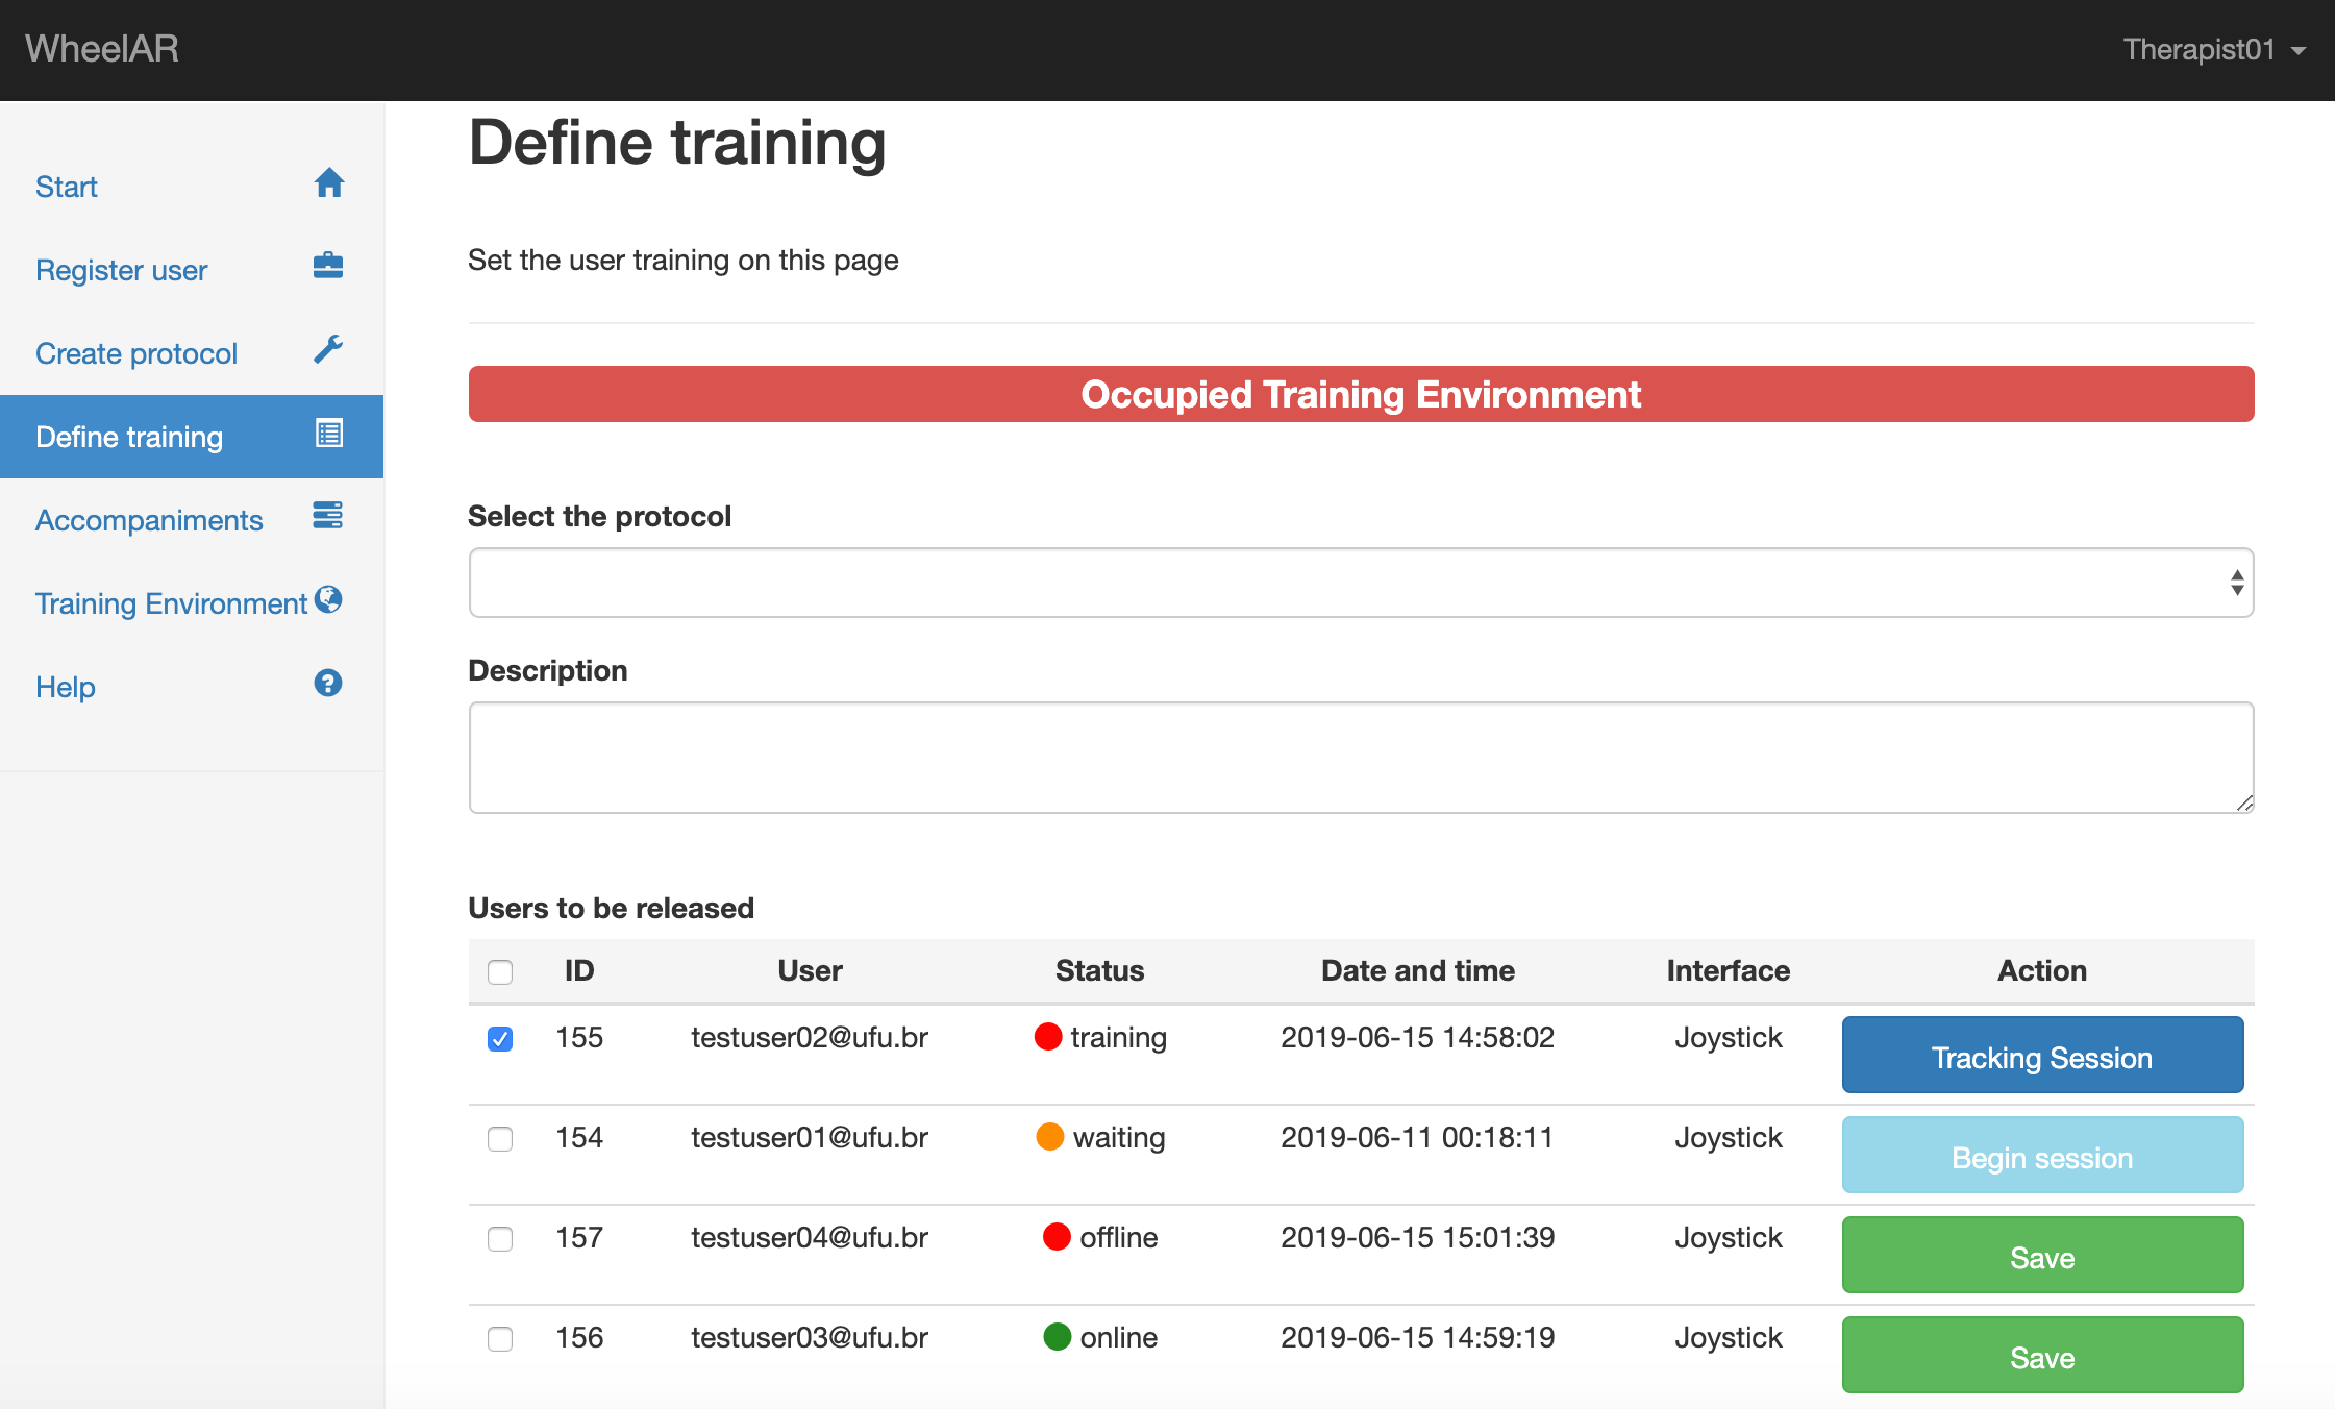
\includegraphics[width=1\linewidth]{img/cap5/tDefineProtocol01}
%\caption{Define training protocol} \label{fig:tDefineProtocol01}
%\end{center}
%\end{figure}
%
%From the SD action (Figure \ref{fig:UMLSD-TherapistWebCase04}) all steps implemented in this UC are detailed and explained on user guide in Appendix \ref{sec:appDefineProcotol}. After the action ``Define training'' is chosen on the menubar, three different Java code blocks are embedded on ``create\_protocolo.jsp'' file and executed before the therapist starts with his actions.
%
%The first one is responsible for checking if the training environment status. When the environment status is ``Occupied'', the ``Begin session'' button is disabled, until training in session in progress has finished. 
%
%\begin{lstlisting}[frame=single,language=Java]  % Start your code-block
%
% //Checking if there are any users in training
% Integer qtd = 0;
% rs = st.executeQuery(select COUNT(userID) as Qtd from patientTH 
%      where status='training');
% if (rs.next()) 
%   {
%   qtd = rs.getInt("Qtd");
%   if (qtd > 0){%>
%     <h3><label class= label label-danger center-block for=
%     "statusEnvironment">Occupied Training Environment</label>
%     </h3> <% }
%   else { %>
%    <h3> <label class= label label-success center-block for=
%    "statusEnvironment">Free Training Environment</label>
%    </h3>
%    <% }
%  }
%\end{lstlisting}
%
%The second one check if in the current session, the therapist already defined a training protocol, which means, he intends to start a new session. Thus, the ``Select the protocol and Description'' fields are hidden until the therapist accomplishes the following session. However, if none protocol were previously defined, another embedded Java code block is executed, retrieving from the database the protocol and activities list. 
%
%The third one is responsible for list all training request by the users on charge of this therapist.
%
%The last actions were updated only on the front-end. However, when a training protocol is selected by the therapist, an Ajax\footnote{https://developer.mozilla.org/en-US/docs/Web/Guide/AJAX/Getting\_Started} Script is also embedded in this file, request from a GET method, the protocol description. The next ``Track session, Begin session and Save'' actions are handle by ``ServletMain'' that filters each one by button action, proceeding just like described in SD action (Figure \ref{fig:UMLSD-TherapistWebCase04}).
%
%Based on training ID where the ``Save'' button is pressed, basic information like protocolID is updated on table assesTH. All information related to the protocol (tasks and virtual objects list) and the user profile are updated on the current session and redirect to the same view page again. 
%
%When the ``Begin session'' button actions are received on ``ServletMain'', its only redirects the therapist to the view page ``Start streaming'' (stored as startstream.jsp). This action is remotely performed only from the training site and the implementation details is describe in Section \ref{sec:startStreaming}. 
%
%After a training session has initiated, the ``Tracking session'' action can be requested and ``ServletMain'' redirects the therapist to the waiting view page presented in Section \ref{sec:waitingVP}. As a training session is already defined, it redirects the therapist to the ``Therapist ViewPort'' view page shown in Figure \ref{fig:ViewPortTherapist} that were implemented similar to ``User ViewPort'' presented in Section \ref{sec:viewPortUser}.
%
%\begin{figure}[!hbt]
%\begin{center}
%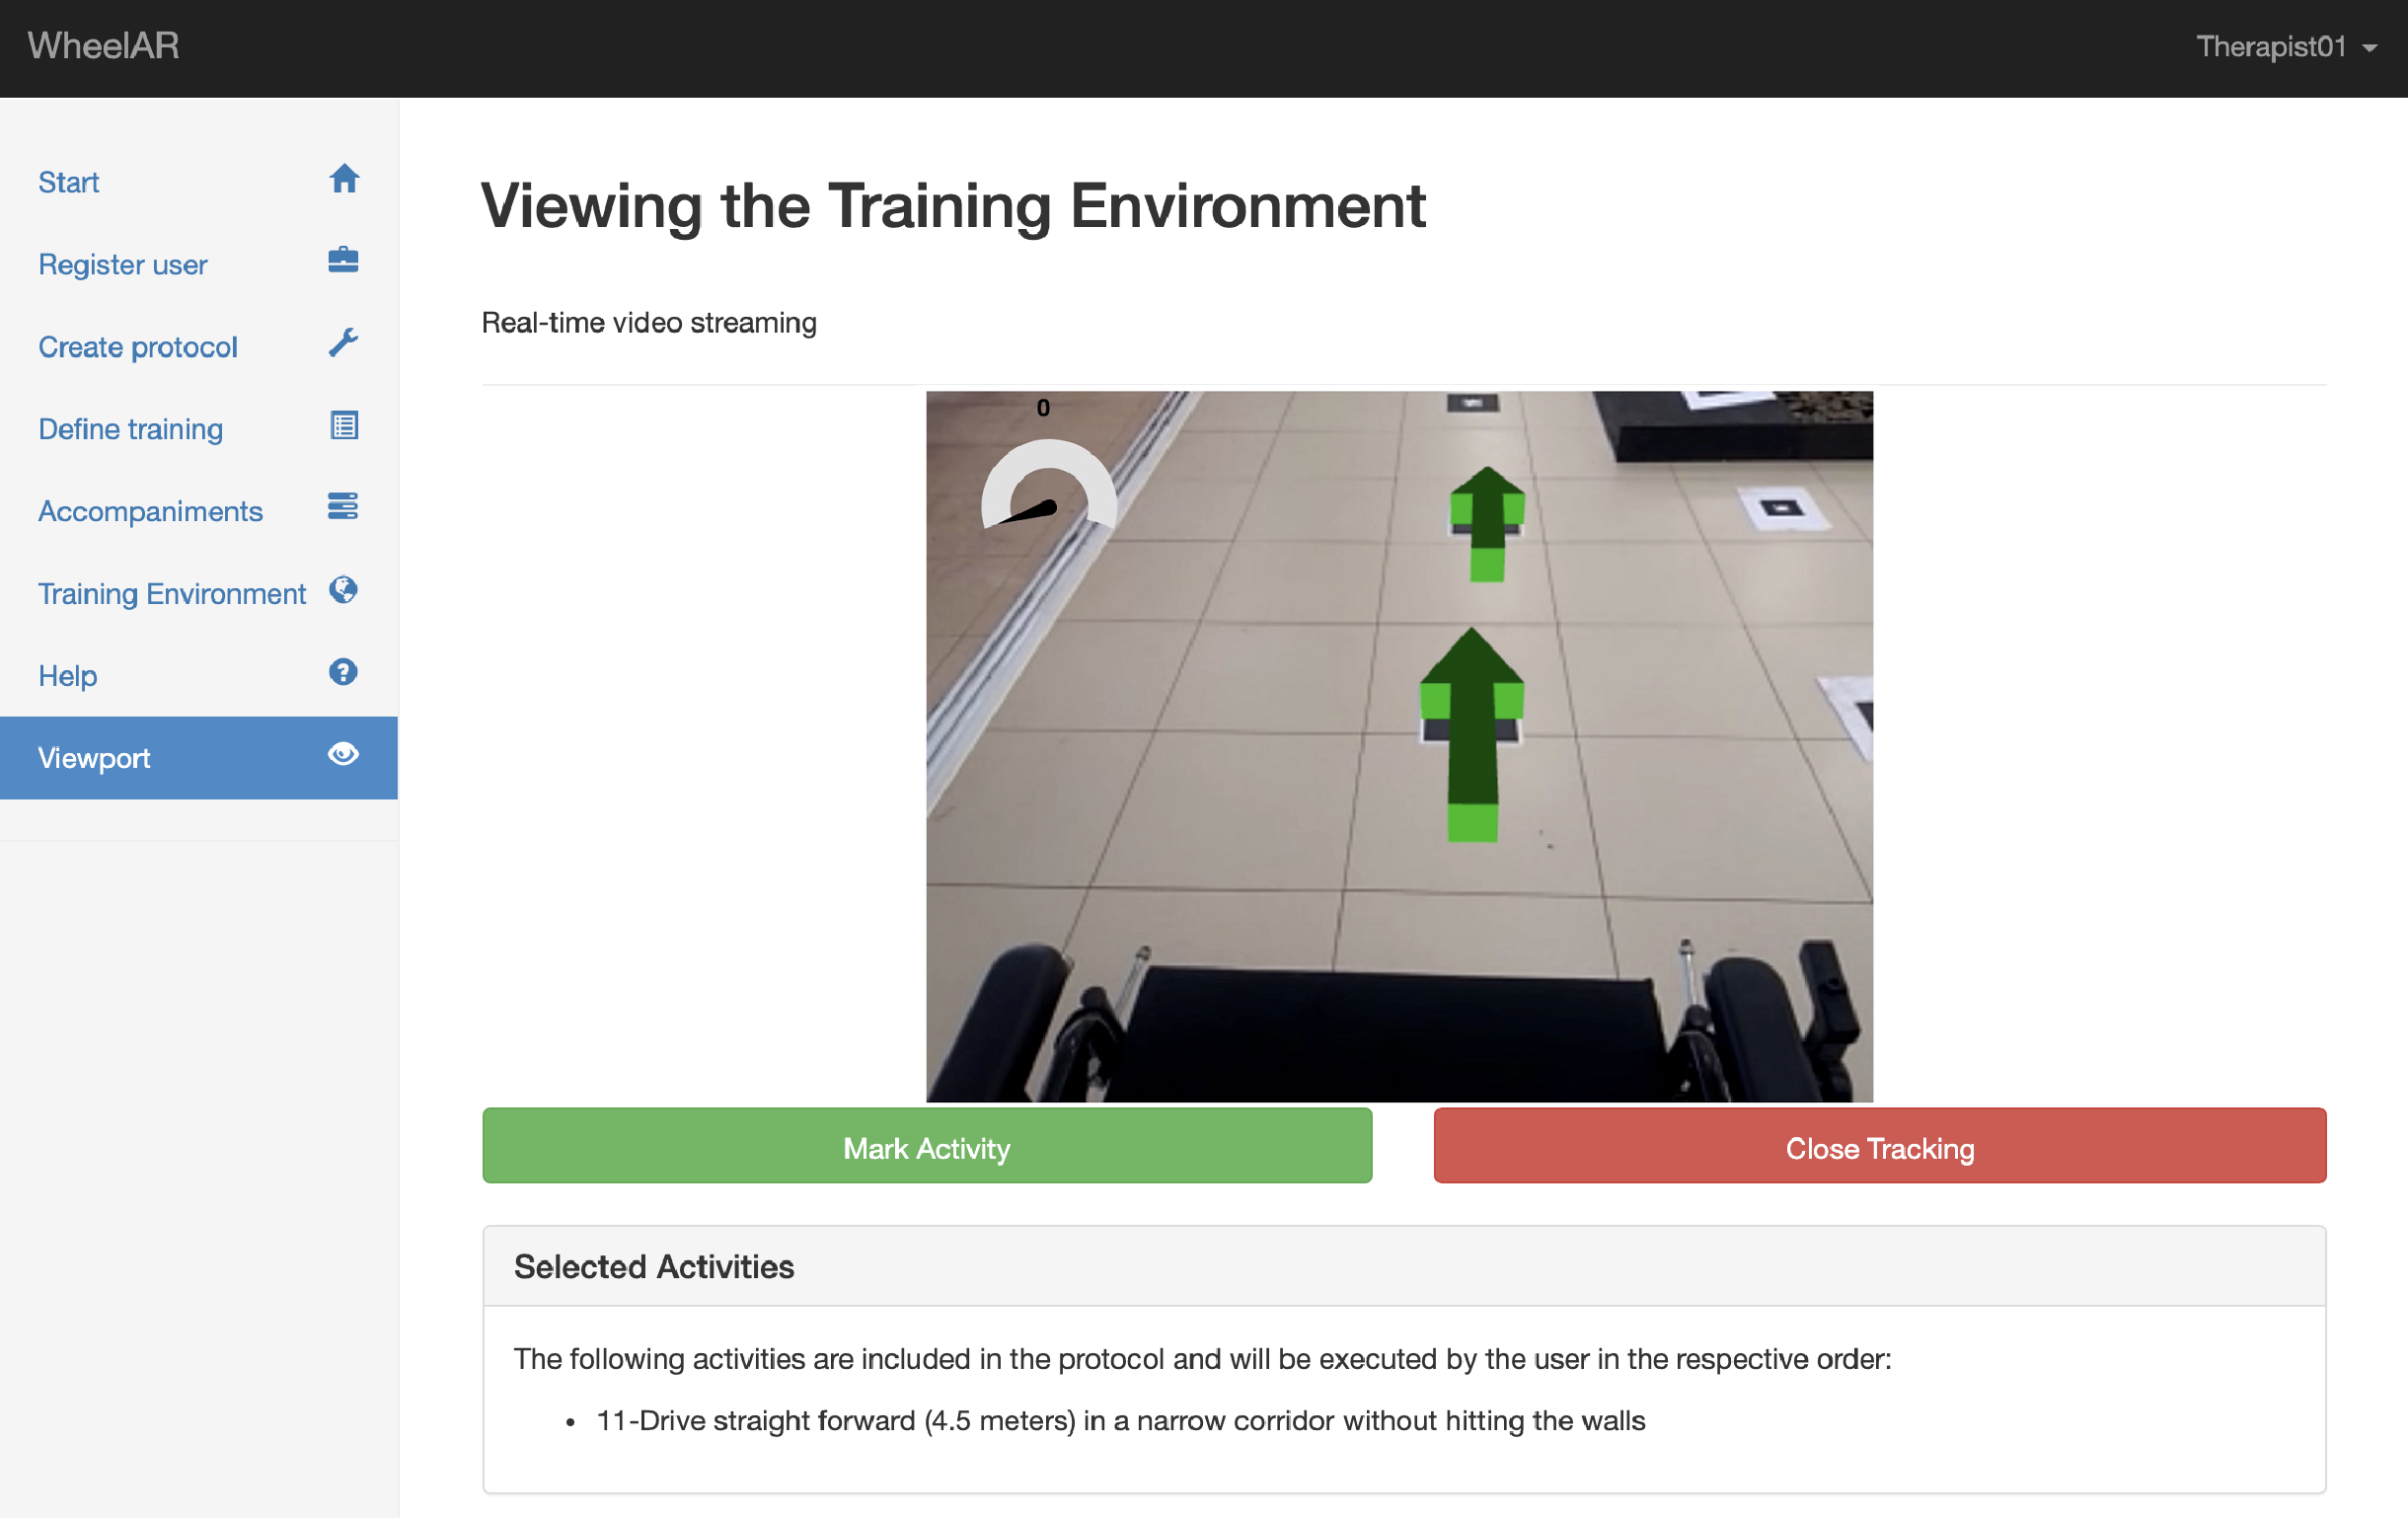
\includegraphics[width=1\linewidth]{img/cap5/tViewPortTherapist}
%\caption{Tracking session and Therapist ViewPort page} \label{fig:ViewPortTherapist}
%\end{center}
%\end{figure}
%
%
%Thus, it allows having augmented feedback from the training site. Furthermore, ``ViewPort'' view page has the button action dynamically update according to the user profile and also brings the activity list to be performed by the user on bottom. For the therapist profile, two different button actions are included (``Mark Activity and Close training''). 
%
%The ``Mark Activity'' button action is very important, once the commandStamps and timeStamps are stored on assessTH table to ensure a future evaluation. Each training protocol can have different tasks number. Then, to mark when a performed task has accomplished by the user, this button action was implemented and its function were attached with ``markTask.js'' file stored in ``js'' folder. It's a simples action, when this button is pressed, a specific command is sent to ``ServletCommand'' which is responsible for handling it, a ``-'' is inserted into the command and timestamp string allowing to apply a separated measure for each task later. 
%
%Therefore, when the user concludes the training session, the therapist trigger the ``Close training'' handled by ``ServletMain''. Before being redirected to the next UC action ``Evaluate training'', the data stored during the user's training session is processed. Information such as the participant and protocol name, execution date, beginning and end training time, session time, commands amount and elapsed time for each activity are separated and updated in the session.
%
%\subsubsection{Evaluate training}
%
%Beyond allowing the PW user to perform telerehabilitation activities as they do in rehabilitation centers, the therapist must be enabled to perform their assignments at a distance. Also, creates individualized training activities, he must be able to assess the user's performance after the training section. Thus, an adaptation to the PMRT assessment form was implemented (stored as avaliar\_treinamento.jsp), as shown in Figure \ref{fig:tEvaluateTraining} to ensure it.
%
%\begin{figure}[!hbt]
%\begin{center}
%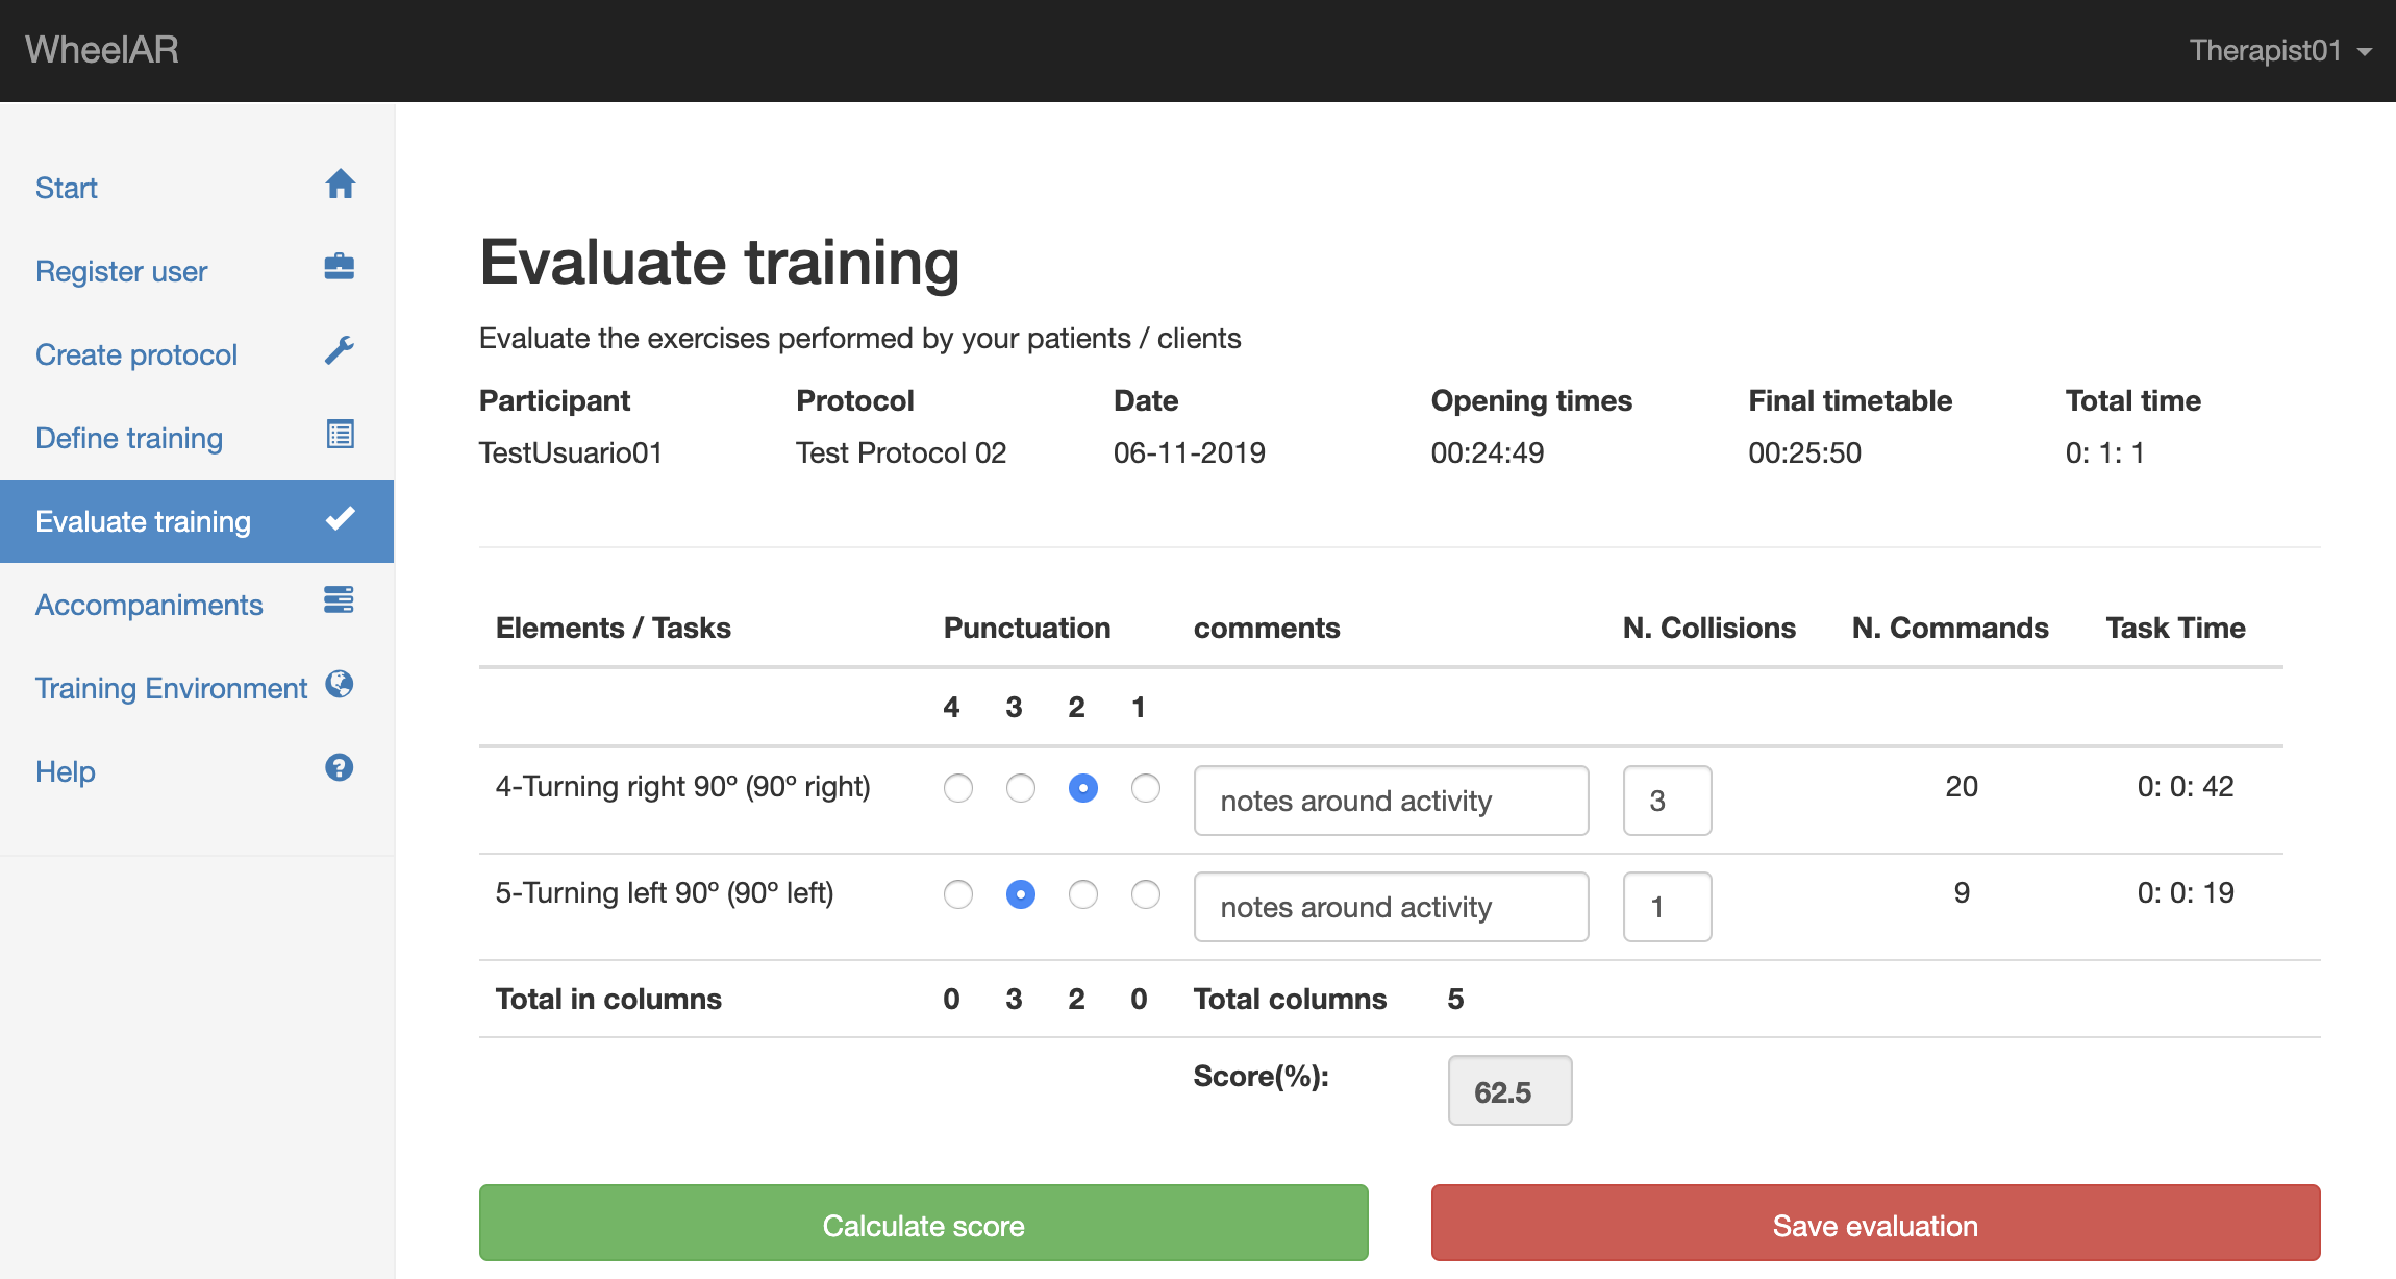
\includegraphics[width=1\linewidth]{img/cap5/tEvaluateTraining}
%\caption{Adapted PMRT Evaluation Form} \label{fig:tEvaluateTraining}
%\end{center}
%\end{figure}
%
%The PMRT Assessment Form is automatically generated on onload view page process by an embedded Java Code, responsible for collecting all training data on the session and render the evaluation form with the ``Calculate score and Save evaluation'' button action. 
%
%The therapist has to fill out the comments around, collision number and then choose a relative score for each activity. Before saving the evaluation, the ``Calculate score'' button is triggered to update the score, where a ``onclick'' JavaScript action is attached. Thus, when the ``Save evaluation'' action button is pressed  the ``ServletMain'' update the assessment information on the ``assessTH'' table and system redirects user for the next therapist UC action ``Anottations''. 
%
%\subsubsection{Annotations}
%
%After the redirect action to the ``anotacoes.jsp'' view page ( Figure \ref{fig:tAnnotations}) that implements the last task to be concluded by the therapist of the user training session evaluation.
%
%\begin{figure}[!hbt]
%\begin{center}
%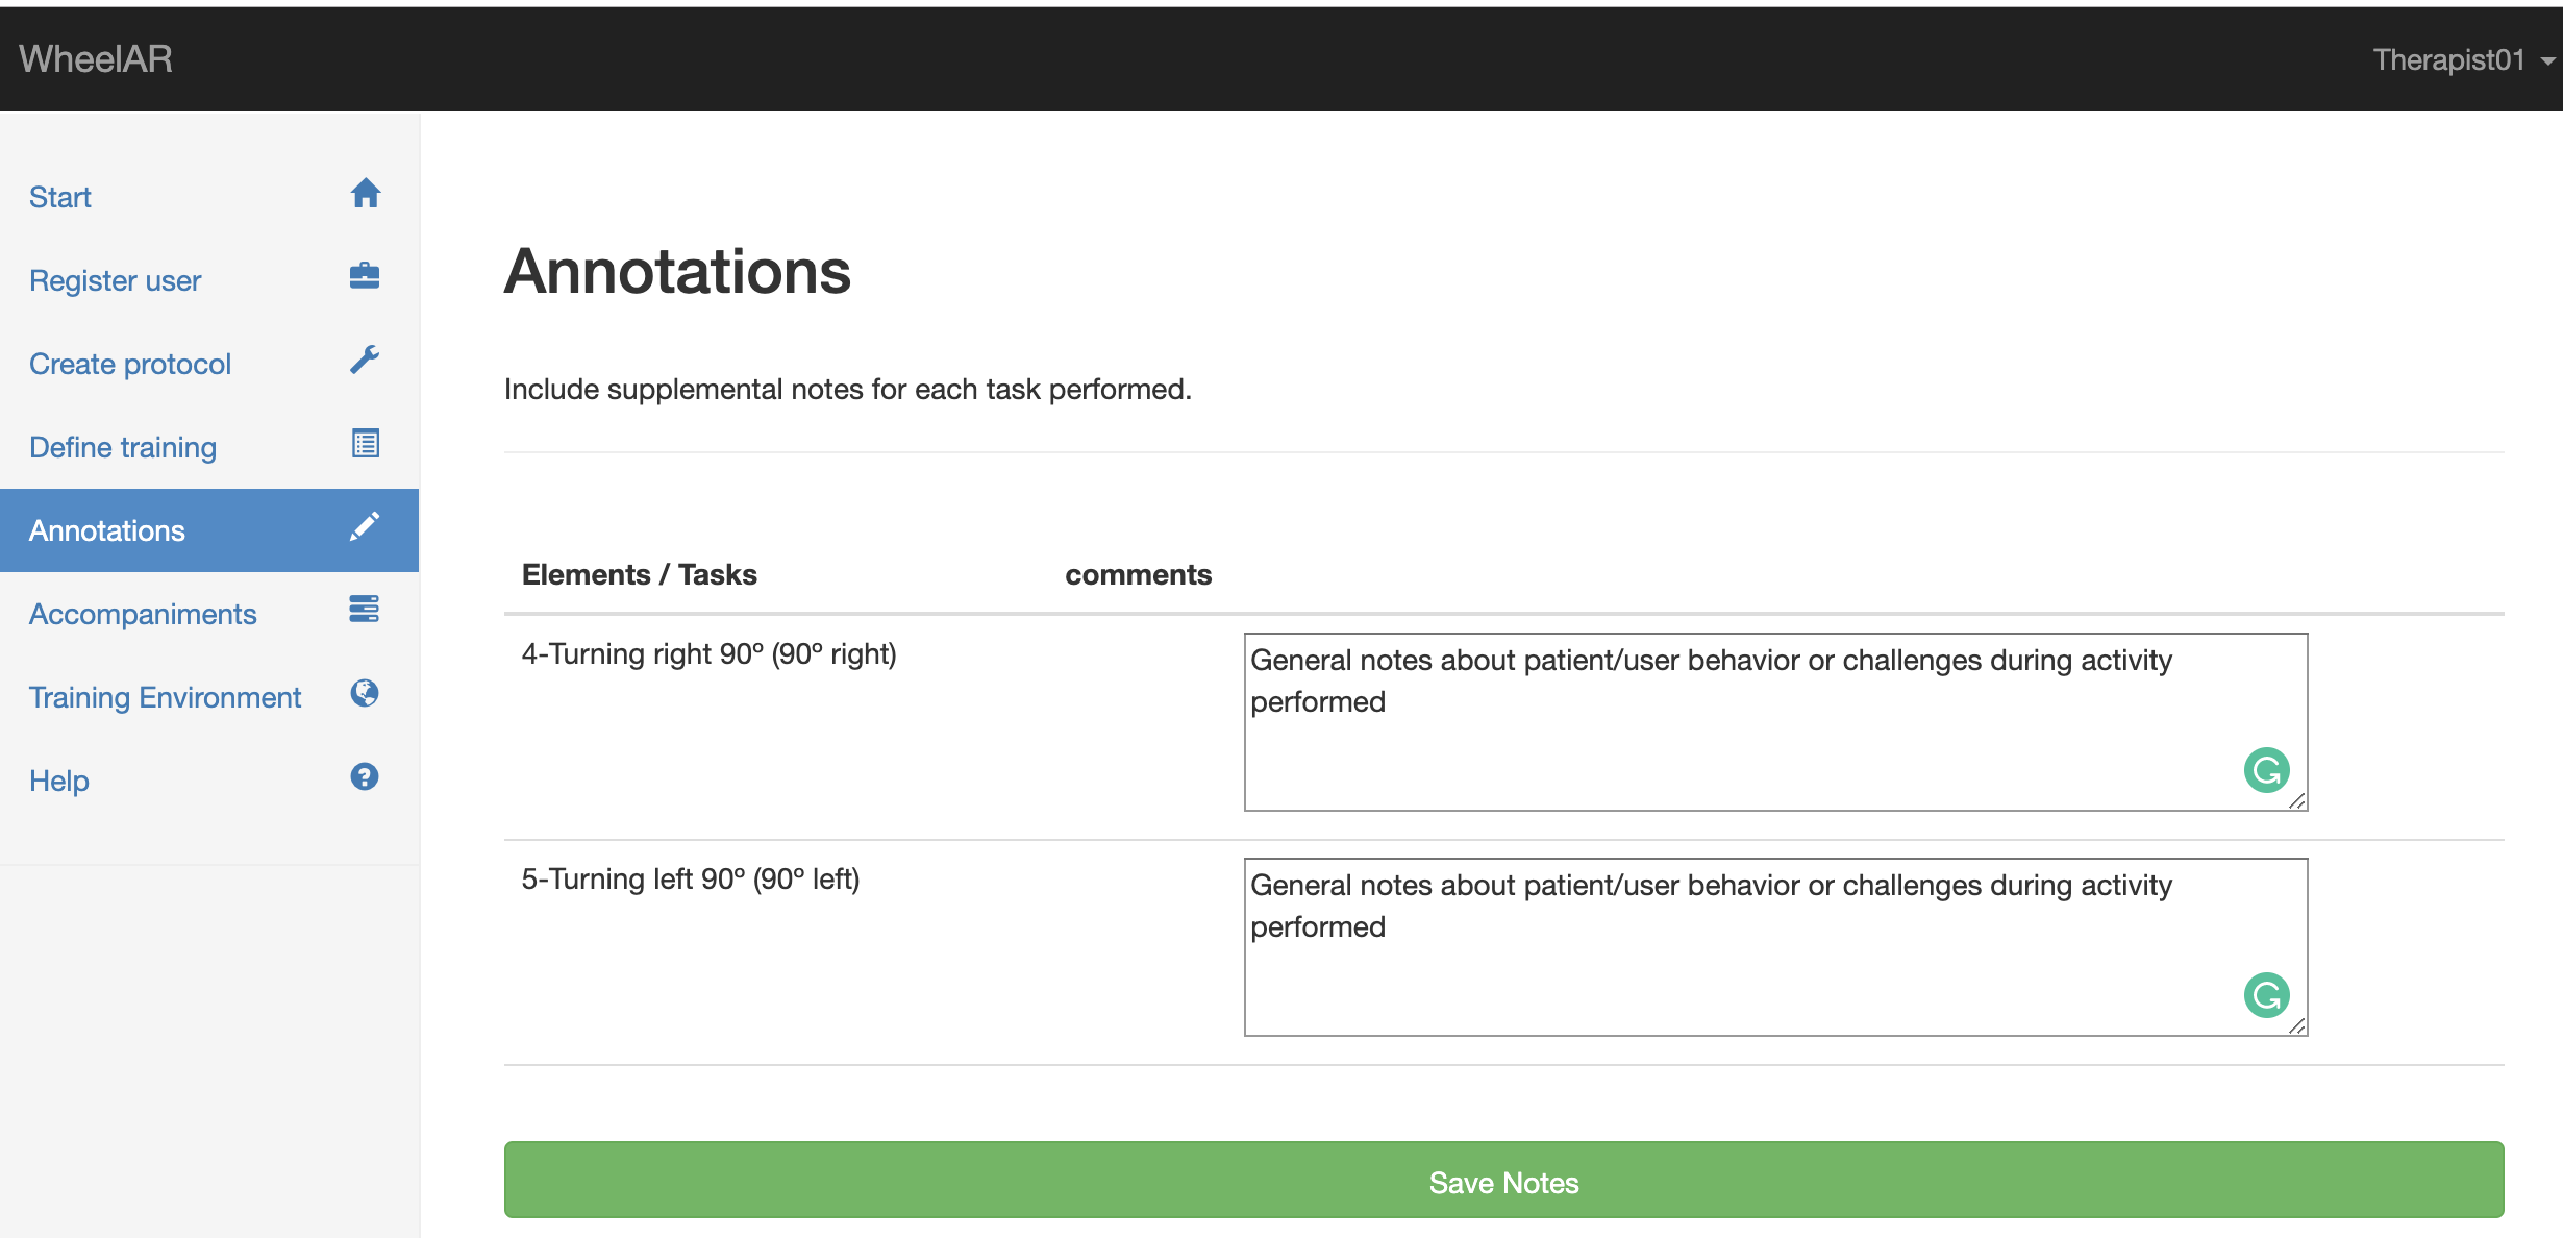
\includegraphics[width=1\linewidth]{img/cap5/tAnnotations}
%\caption{General and clinicians notes around the user evolution} \label{fig:tAnnotations}
%\end{center}
%\end{figure}
%
%On onload view page process, another embedded Java code block is executed. It retrieves from session variables the current training tasks performed by the user. Allowing the therapist to take notes related to the user evolution, and after, pressing the button ``Save notes'' another POST action is sent to the ``ServletMain''. It recognizes the request and stores the information filled out by the therapist on the ``historyTH'' table. 
%
%Then, redirects the therapist to the main page from where he is able at any time to follow the user's evolution history.  
%
%
%\subsubsection{Accompaniments}
%
%In order to provide to the therapist clues of the user evolution after the training sessions, the ``Accompaniments'' view page (stored as a acompanhamento.jsp) is presented by Figure \ref{fig:tGenerateChart02}. This therapist UC action can be accessed at anytime because all training metrics are merged in a bar chart graph generate in real-time.  
%
%\begin{figure}[!hbt]
%\begin{center}
%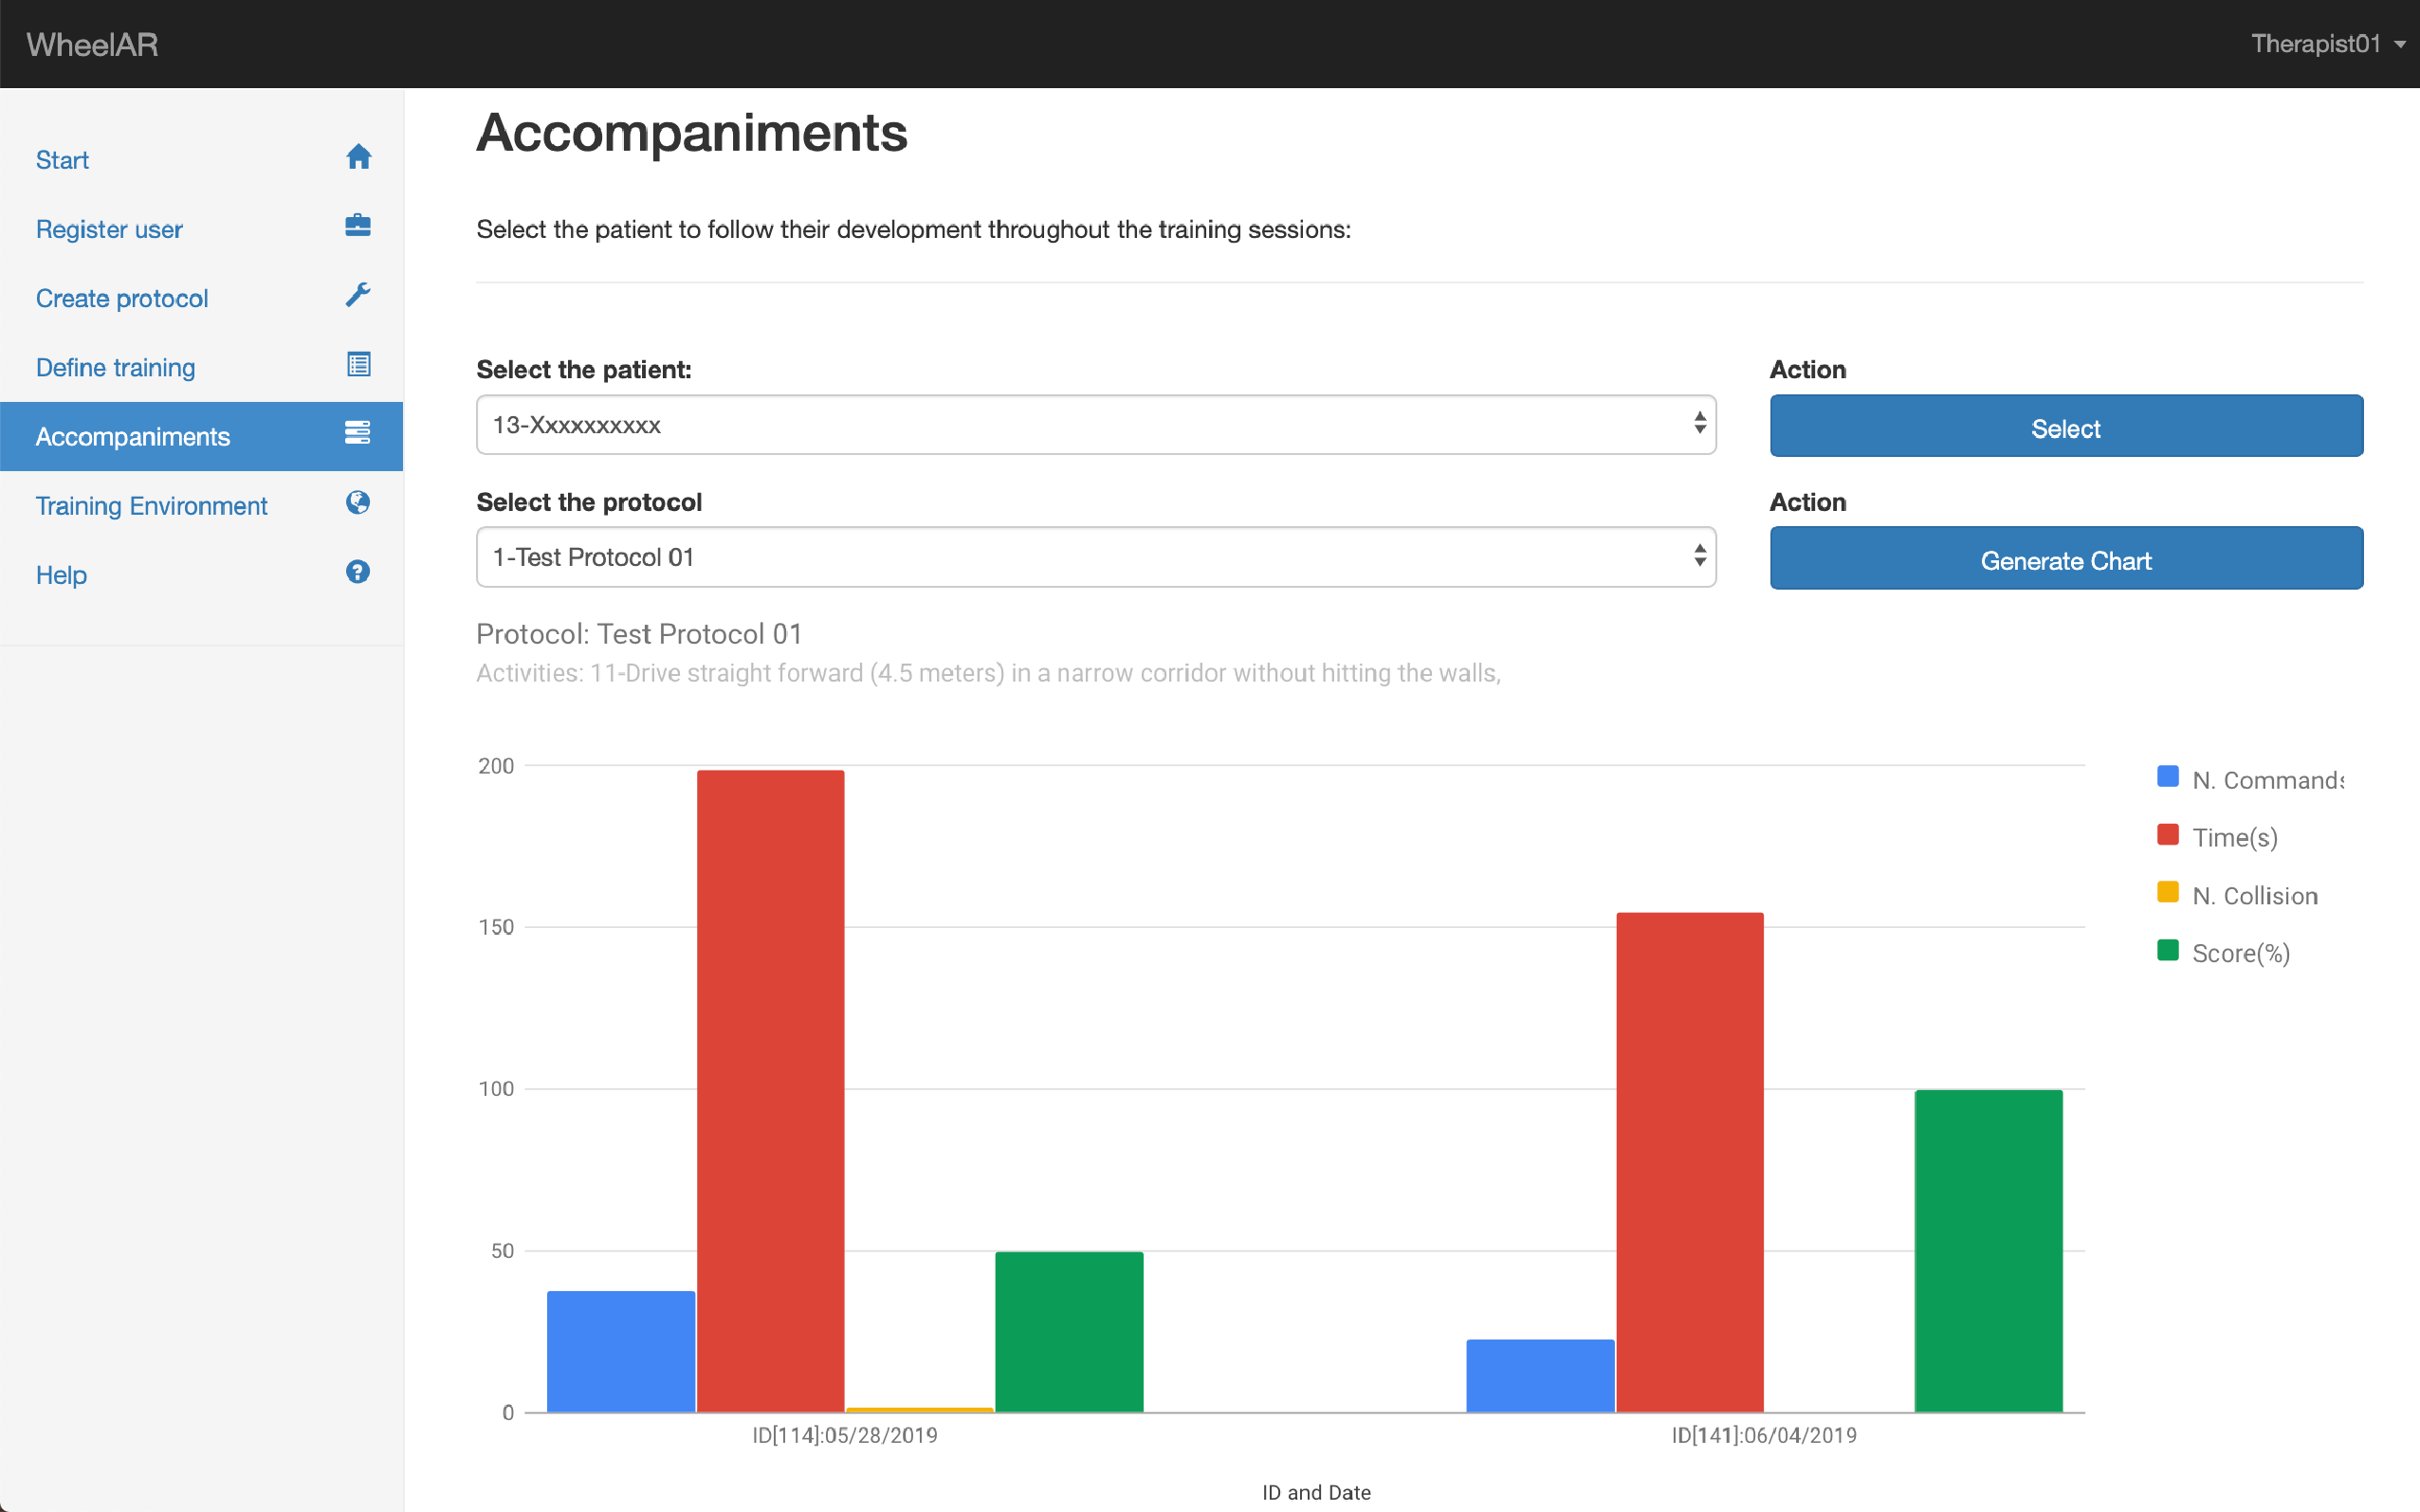
\includegraphics[width=1\linewidth]{img/cap5/tGenerateChart02}
%\caption{Comparative chart users training protocols performed} \label{fig:tGenerateChart02}
%\end{center}
%\end{figure}
%
%Firstly, an embedded Java code responsible to fill the ``Select the user'' list is executed on onload view page process. To generate a chart, the therapist has to select a user on the list and press the ``Select'' button action that is sent to the ``ServletMain''. The servlet retrieve from the ``assessTH'' table all training records and respective metrics and update it on session. Now, the therapist is able to select from ``Select the protocol'' list all training sessions performed and to preview the chart the ``Generate chart'' button have to be pressed.
%
%Using the ``Google Charts''\footnote{https://developers.google.com/chart} free JavaScript library, it is easy to generate a different kind of graphics information. Then, following the library documentation all session data is properly used to fill each function and render the visual graphics. 
%
%In addition to this graph, information about the SI or excitation from the biosignals allows the evaluation of the emotional state of the same, helping also in the understanding of the real difficulties and observing the overcoming of them after each session. 
%
%\section{Training site}
%\label{sec:impltrainingsite}
%
%It is from this site that a large part of the telerehabilitation process takes place. The user can control the PW, safely increasing their driving skills remotely.  The therapist can define and create protocols remotely,  that the user will execute, if necessary, interact with the PW. Also, simultaneously they preview augmented feedback from the training to be conducted. For this reason, the implementation details are divided into two parts: opening and transmitting the video stream and PW embedded program for remote control.
%
%\subsection{Start streaming}
%\label{sec:startStreaming}
%
%As previously mentioned in Section \ref{sec:definedProtocol} the action ``Begin session'' interfaced through the page ``Start Streaming'' (Figure \ref{fig:tStartStream}) is performed only from the training site. 
%
%\begin{figure}[!hbt]
%\begin{center}
%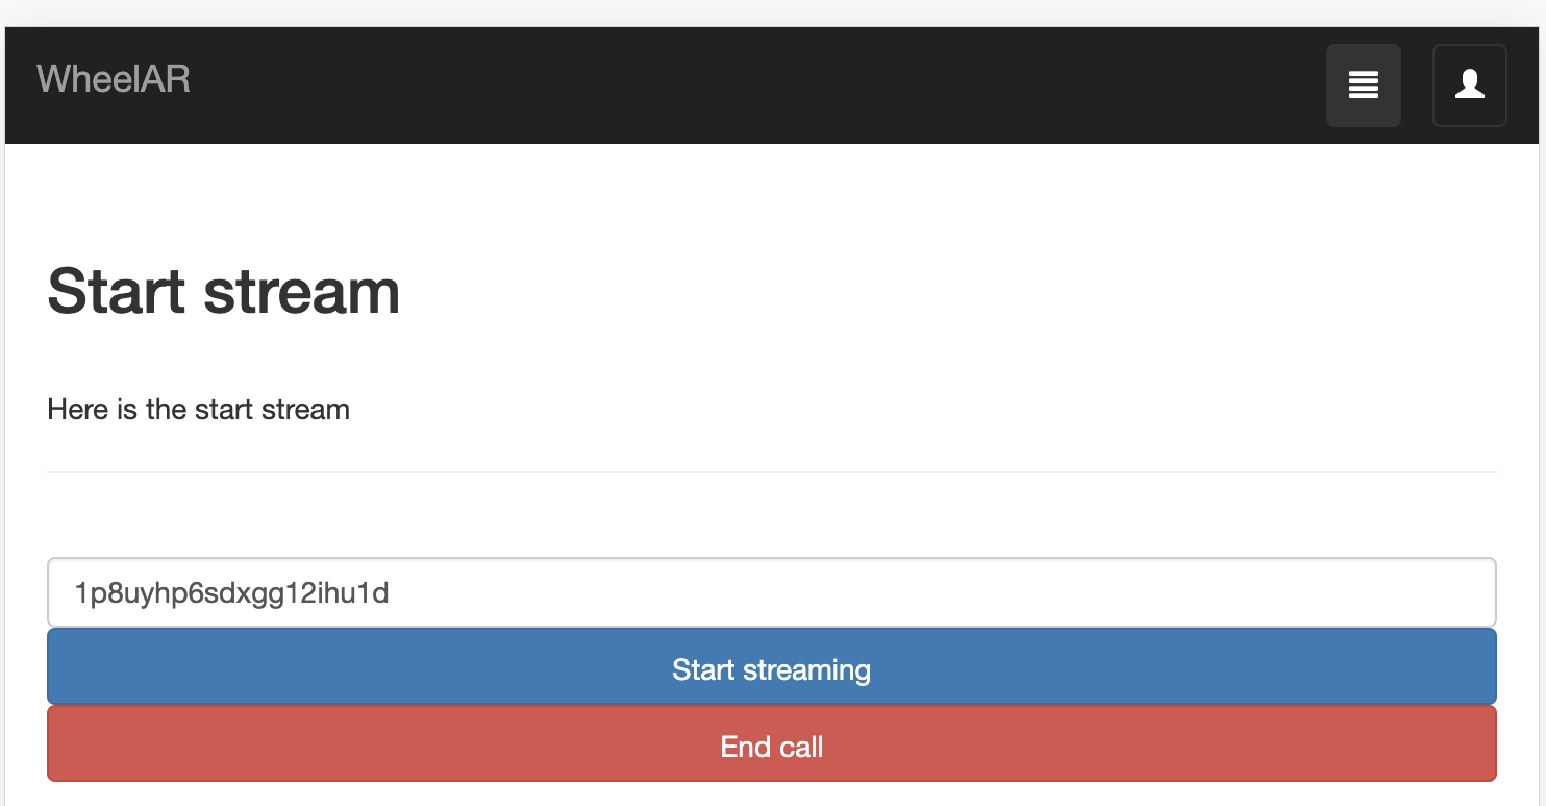
\includegraphics[width=0.7\linewidth]{img/cap5/tStartStream}
%\caption{Start streaming therapist page} \label{fig:tStartStream}
%\end{center}
%\end{figure}
%
%The buttons displayed on the page, as well as the text field that displays the code automatically generated for connecting to the room, are demonstrated in the HTML code snippet.
%
%
%\begin{lstlisting}[frame=single,language=Java]  % Start your code-block
%
%<div class="row">
%  <div class="col-md-6">
%   <input type="text" id="room-id" value="abcdef">
%  </div>
%  <div class="col-md-3">
%   <button id="open-room">Start streaming</button>
%  </div>
%  <div class="col-md-3">
%   <button id="" onclick="endStreaming()">End call</button>
%  </div>
%</div>
%<div class="hidden text-center container" id="videos-container">
%</div>
%
%\end{lstlisting}
%
%To implement the WebRTC streaming, same libraries from ``js/dist/'' and also ``js/dev'' (getHTMLMediaElement.js and adapter.js) were used. Before the ``Start streaming'' action button is pressed, where a JavaScript event click is attached, an automatic video device detection was implemented.  It is needed because there is a difference in detecting devices on smartphones (which have more than one device (front or back)) to a desktop or notebook (which has only one video device (front)). The code snippet below exemplifies the actions implemented. \newline
%
%\begin{lstlisting}[frame=single,language=Java]  % Start your code-block
%
%var videodeviceid;
%var videoList=[];
%
%navigator.mediaDevices.enumerateDevices().then(gotDevices).
%  catch(handleError);
%function gotDevices(deviceInfos) 
%{
%  for (var i = 0; i !== deviceInfos.length; ++i) 
%   {
%    //implements a video and audio devices detection
%    //add devices detected to the videoList vector
%   }
%  if(DetectRTC.isMobileDevice)
%   {
%   //retrieve the second element from the videoList
%   }
%  else
%   {
%   //retrieve the first element from the videoList
%   }
%}
%\end{lstlisting}
%
%Using the ``adapter.js'' library is possible to enumerate audio and video inputs. The deviceInfos variable has this information and using a repeating structure; it is possible to filter and store on videoList vector, those are interested. Then using the ``DetectRTC class'' from the ``getHTMLMediaElement.js'' library, it is possible to know if the user is using a desktop, notebook, or smartphone and select the specific video device. When it is a ``MobileDevice'', the second element of the videoList selected to use the back camera device.
%
%To start a shared video call, the `` Start streaming '' button must be pressed. Through the click event associated with it, another function in JavaScript is executed. It displays the video element previously hidden, because an HTML canvas object for rendering the video, will be returned. Next, the room-id randomly generated, and also, the video-source-id of the streaming, are retrieved. Through the ``socket.io.js '' library, a new ``WebSocket'' is created to wait for the connections to be established through a shared link. After this process is completed on the front-end, the video is updated in <div> ( videos-container), another JavaScript function that executes an HTTP POST method, sends the generated room-id to the ``ServletWebRTC''. Thus, the servlet proceeds with updates process: the connection training link and release column to ``true'' in the table ``assessTH'',  the user status for ``training''  in the table ``patientTH''. These updates allow the commands to be forwarded to the training site and metrics measuring by the ``ServletCommand''. 
%
%
%\subsection{PW Control}
%\label{sec:pwControl}
%
%To ensure that the PW can be remotely operated, embedded software has been implemented. This software works as a polling IO process. Then, it is possible to receive the commands through WiFi, start the engines properly and update their PW speed information.
%
%The first step is to change the Dlink DWR-922B 4G router modem settings so that it correctly forwards the received packets from the external network to the internal network. This feature is known as the ``port forwarding'' setup (Figure \ref{fig:pfnDiagram}).
%
%\begin{figure}[!hbt]
%\begin{center}
%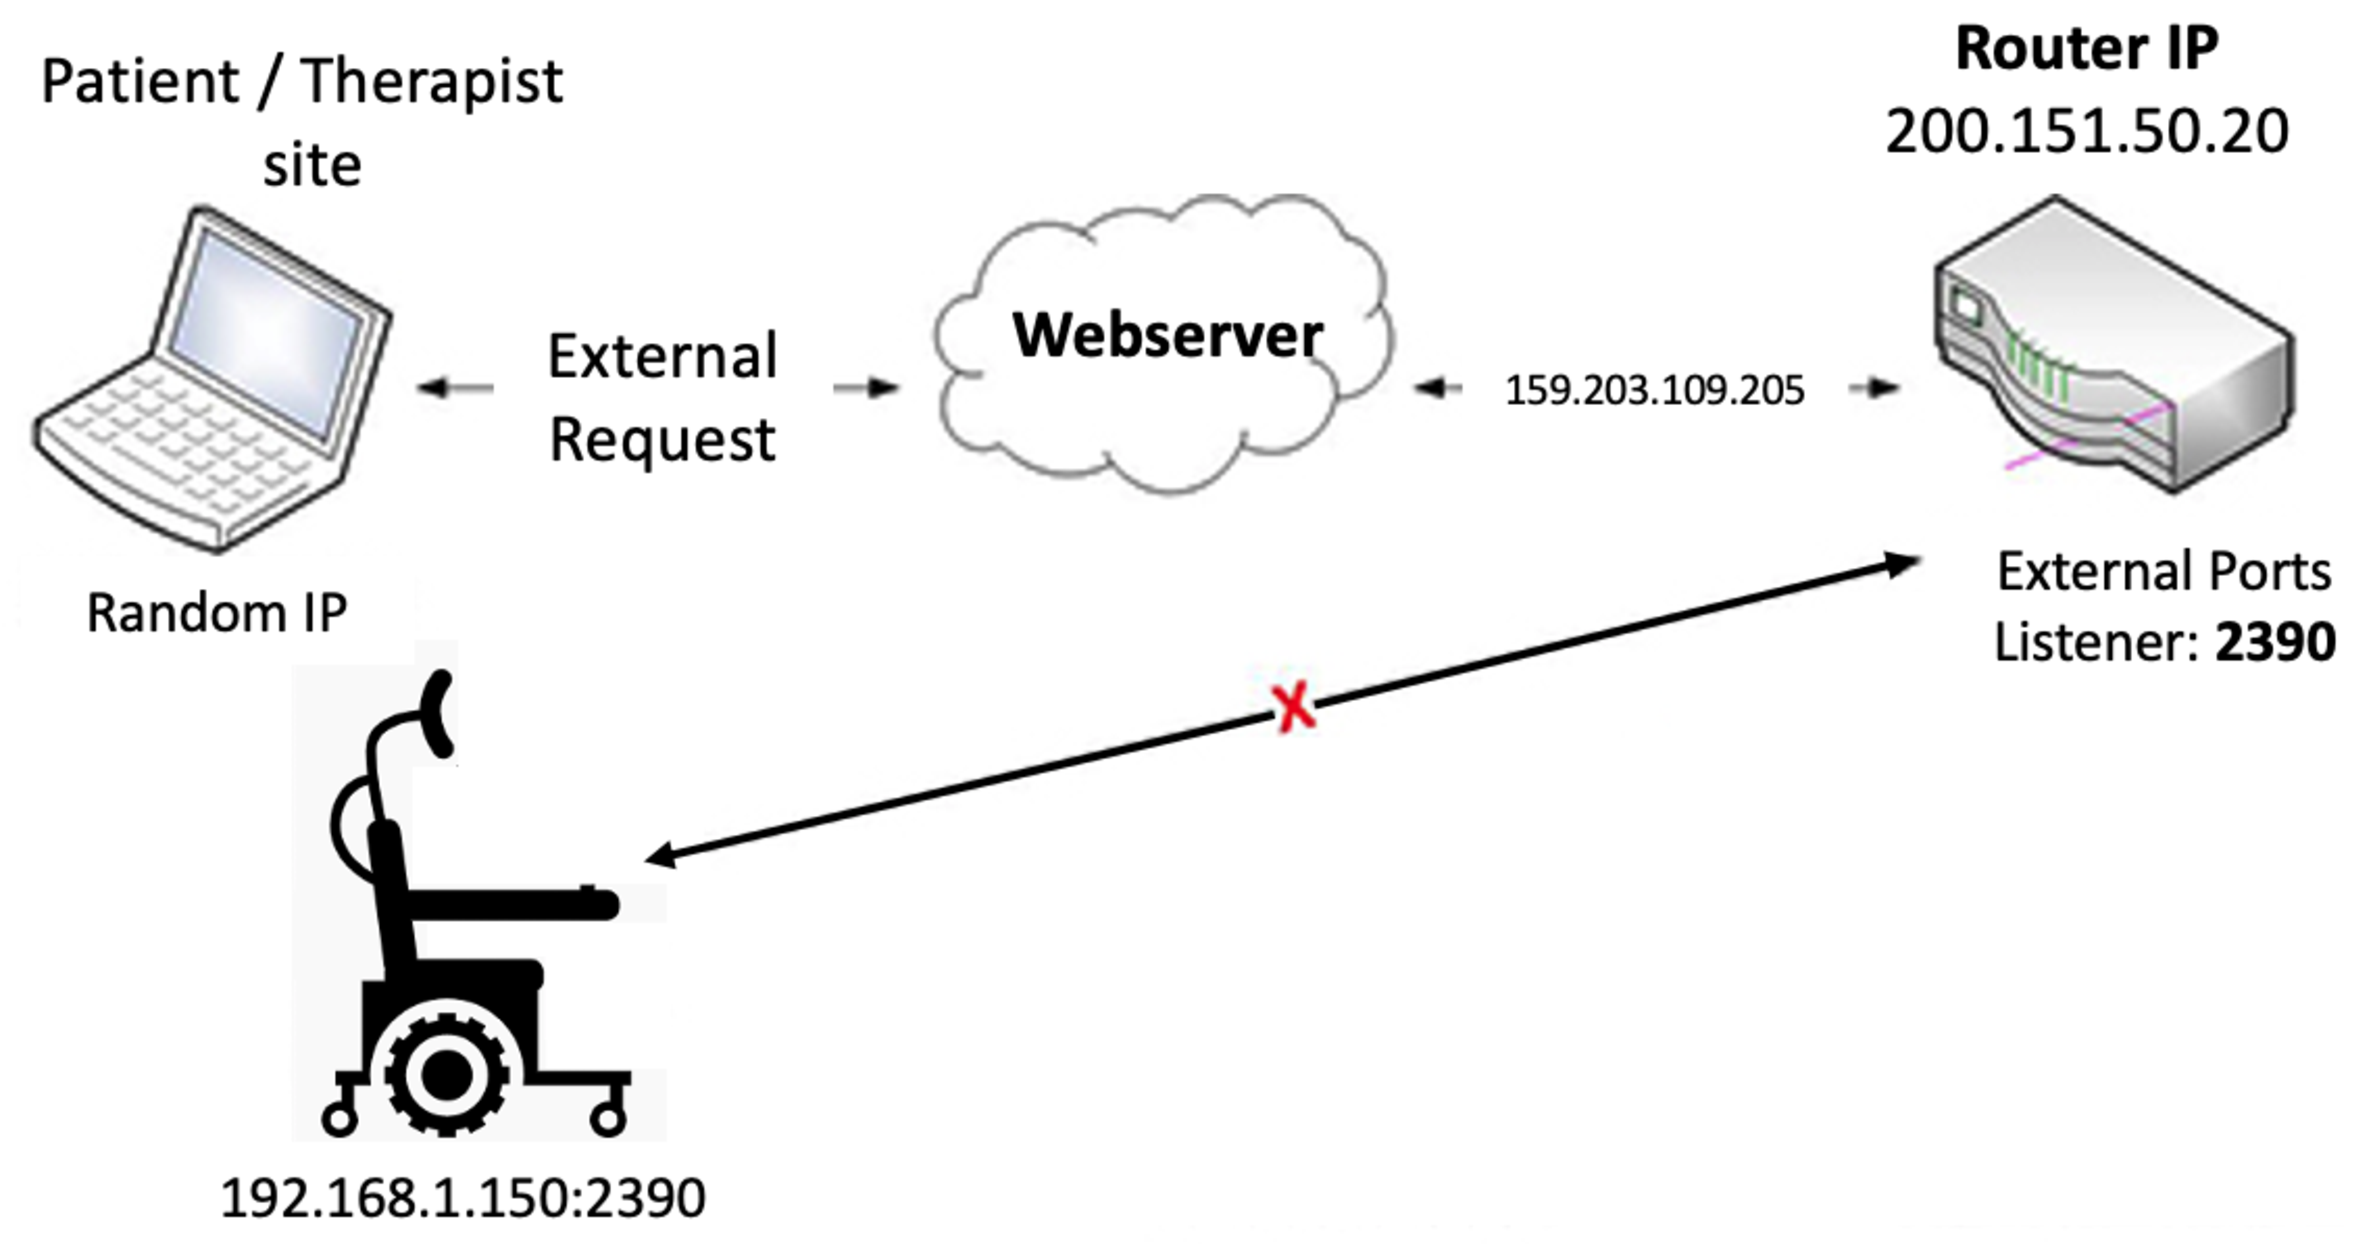
\includegraphics[width=0.8\linewidth]{img/cap5/pfnDiagram2}
%\caption{General Port Forwarding Network Diagram} \label{fig:pfnDiagram}
%\end{center}
%\end{figure}
%
%Following the router's user manual, installation is straightforward. For this, it is necessary to define a name for the routing, the public port as (2390), traffic type as UDP, define the Arduino internal IP and the internal port as (2390). With this, the embedded software is ready to receive commands and transmit information with the web server. 
%
%Before describing part of the code that was implemented to perform the control, emergency stop and PW speed update, it is necessary to set up all the microcontroller resources to be used, such as external interrupts and digital pins. The code snippet below describes this configuration.\newline
%
%\begin{lstlisting}[frame=single,language=Java]  % Start your code-block
%  
%  //SETTING UP PW PINS
%  pinMode(2, OUTPUT); // PW control 2 pin
%  pinMode(3, OUTPUT); // PW control 3 pin
%  pinMode(4, OUTPUT); // PW control 4 pin
%  pinMode(5, OUTPUT); // PW control 5 pin
%  pinMode(6, OUTPUT); // PW control 6 pin
%
%  //SETTING UP RPM SENSOR
%  pinMode(30, OUTPUT); //VCC Pin
%  pinMode(32, OUTPUT); //GND Pin
%  digitalWrite(30, HIGH); //Turning VCC on
%  digitalWrite(32, LOW);  //Turning GND on
%  
%  //SETTING UP External Interrupt (Speed Sensor)
%  attachInterrupt(digitalPinToInterrupt(Speed_sensor_interrupt), 
%   debounceInterrupt, CHANGE);
%
%  //SETTING UP WIFI CONNECTION
%  setupWifiConnection();
%\end{lstlisting}
%
%The five settings up PW pins described will be used by a function responsible for verifying which command (string) received from the server and adjusting different voltage values for each pin, promoting the proper activation of the PW.
%
%
%The RPM sensor configurations pins were performed due to a limitation of the microcontroller pins number (VCC and GND)  necessary for feeding the sensor. Next, a function configuration for treating external interrupts detection by the infrared sensor reflection variation was defined. 
%
%However, without the WiFi Shield configuration, which is responsible for handling receiving and sending information through the router, none of this is of use. For this, an UDP data communication\footnote {https://www.arduino.cc/en/Tutorial/WiFiSendReceiveUDPString}  example was used, provided by the manufacturer to deals with it, is represented by the setupWifiConnection() function.
%
%The polling IO process is implemented by the ``void loop()'' function.\newline
%
%\begin{lstlisting}[frame=single,language=Java]  % Start your code-block
%  
%void loop() {
%  checkRPMValues(); //Checking sensor state
%
%  // if there's data available, read a packet
%  int packetSize = Udp.parsePacket();
%  if (packetSize) {
%    timeIn = millis(); // Storing the incoming packet timestamp
%
%    // read the packet into packetBufffer
%    int len = Udp.read(packetBuffer, 255);
%    if (len > 0) {
%      packetBuffer[len] = 0;
%    }
%    lastCommand=packetBuffer[1];
%    updateWheel_kmh();
%    deltaTime.concat(wheel_kmh);
%    deltaTime.toCharArray(packetBuffer, deltaTime.length() + 1);
%    //reply, to the IP address and port that sent us the packet
%    Udp.beginPacket(Udp.remoteIP(), Udp.remotePort());
%    Udp.write(packetBuffer);
%    Udp.endPacket();
%    deltaTime = "";
%  }
%  activateMotors(lastCommand);
%  securityStop(timeIn);
%}
%\end{lstlisting}
%
%Continually, the revolutions per minute (RPM) number of the PW is updated,  and also, if there is any data packet received. If it exists, then the received package time is stored, and immediately the package is read. After due checks, the transmitted command value is correctly assigned to the ``lastCommand'' variable, as it will be used to start the PW engines. Thus, the RPM value is converted into kilometers per hour (Km/h). This value is assigned to the received package and forwards it back to the ``ServletCommand'' to update this value into the ``assessTH'' table to allow ``ServletSpeedPW'' to collect valid speed information and update it on the speedometer. Finally, the functions ``activateMotors'' and ``securityStop'' are called to respectively activate the PW engines and if the time without receiving packets is more than three seconds, stop the PW.
%
%
%\section{Final considerations}
%
%This chapter described the implementation details of the proposed system architecture to support telerehabilitation for training PW users, using Augmented Reality techniques. So far, it has been found in the literature no architecture that allows the therapist and users to continue this fundamental process, despite the distance. 
%
%In order to overcome this distance, the WebRTC framework was used to allow even in a different site (therapist and patient) to be connected to the training site. However, it is not just about being connected. It is also needed that the user has a safe and enriching training experience within their conditions. 
%
%For this, it is also necessary for the therapist to be able to use some technological resource that, even at a distance, the user can be guided in a real scenario, performing personalized tasks, and the therapist still is able to evaluate and monitor his development.  For this reason, the use of Augmented Reality techniques is essential for allowing this remote customization where the entire process can be carried out safely. 
%
%Many challenges have been found during this process, since the implementation of the web server responsible for meeting all these demands, so that everyone could use it easily without any program installation and that it could be accessed from any computer with the Internet, is not trivial. The integration of WebRTC with Augmented Reality was challenging as the AR libraries were not prepared to work with remote video sources, and also, with the dynamic 3D objects update in the environment's markers in agreement with therapist definition.
% 
%The development of this architecture is not just the one purpose of this work. But also to demonstrate the architecture capability to afford telerehabilitation. Thus, adaptative and customized training protocols, training evaluation, realistic and safe training conditions were implemented. Eligible users have evaluated the architectural features and the results obtained are presented in the next chapter.